%%%%%%%%%%%%%%%
%shray_sharan@tamu.edu
%%%%%%%%%%%%%%%



\documentclass[SectionMethod, ListStyleI]{TAMUthesis}
%use the line below if you prefer the ChapterMethod, do remember to comment the two lines for Appendix below for correct Appendix format
%\documentclass[ChapterMethod, ListStyleI]{TAMUthesis}
\newcommand{\rom}[1]{\uppercase\expandafter{\romannumeral #1\relax}}
\newcommand{\ignore}[1]{}
%*******************************************
% AREA to claim  Package
%All packages used are declared in TAMUthesis.cls
%For your personal used package, please  app them here, for example
%\usepackage{amsmath}
%\usepackage[labelsep=period]{caption}

%*******************************************
% End of AREA of Using Package
% End of AREA of Using Package
%*******************************************

\numberwithin{equation}{chapter}

%FIX
\sloppy
\hfuzz=6pt
\vfuzz=6pt
\hbadness=2000
\vbadness=\maxdimen

\makeatletter
\g@addto@macro{\appendix}{
  \titleformat{\chapter}[display]{\vspace{1ex}\large\bfseries\centering}{\chaptertitlename\ \thechapter}{0.25pc}{\large}
}
\makeatother

%FIX
\graphicspath{{graphic/}}
\begin{document}



\title{ESTIMATING THE NUMBER OF ACTIVE DEVICES \\ WITHIN A FIXED AREA USING WI-FI MONITORING}
\author{HAI LI}
\TAMUdocument{Thesis} %Record of Study%Dissertation
\TAMUdegree{Master of Science}	% DOCTOR OF PHILOSOPHY
	%MASTER OF ARTS
	%DOCTOR OF EDUCATION
	%DOCTOR OF ENGINEERING
	%DOCTOR OF PUBLIC HEALTH
	%MASTER OF LANDSCAPE ARCHITECTURE
	%MASTER OF MARINE RESOURCES MANAGEMENT
	%MASTER OF NURSING
	%MASTER OF URBAN PLANNING
	%MASTER OF PUBLIC AFFAIRS
	%MASTER OF SCIENCE PUBLIC HEALTH
\ChairOfCommitteeName{Jean-Francois Chamberland}
\CommitteeMemberOneName{Gregory H. Huff}
\CommitteeMemberTwoName{Anxiao Jiang}
\CommitteeMemberThreeName{Tie Liu}	%optional
\HeadOfDepartmentName{Miroslav M. Begovic}
\TAMUgradMonth{December} %August or December, these three options only
\TAMUgradYear{2016}
\TAMUmajor{Electrical and Computer Engineering} % Please refer to the TAMU OGAPS word template for the whole list of Major Subject
%http://ogaps.tamu.edu/OGAPS/media/media-library/Instructions-for-PC-template.pdf
	%only store parameter
\maketitle




\frontmatter
\TAMUAbstractFormat
%%%%%%%%%%%%%%%%%%%%%%%%%%%%%%%%%
%Please keep the line above and only type in below.
%%%%%%%%%%%%%%%%%%%%%%%%%%%%%%%%%

In various situations, there is a need to estimate the number of active devices within a specific area.
This thesis offers one possible approach to accomplish this task.
It focuses on estimating the number of devices in a certain area based on monitoring and processing Wi-Fi metadata, which includes a received signal strength indicator.
To accomplish this goal, four sensing devices are placed at the corners of a rectangular area.
These sensing devices observe and record local data traffic, along with the received signal strength associated with each packets.
For each sensing device, two types of frontends are considered, namely directional and isotropic antennas.
Each sensing device retrieves the received signal strength indicators and the media access control addresses from the 802.11 frames packets transmitted by nearby active wireless devices.
The estimator takes the received signal strength indicators as input and infers the number of active Wi-Fi devices inside the area of interest.
Two algorithms, bayesian and maximum-likelihood, are employed for estimation purposes.
Overall performance is used to compare and contrast the systems implemented with directional antennas and isotropic antennas, respectively.
Theoretical and experimental results both hint at performance improvements when using directional antennas, when compare to standard isotropic antennas.


\TAMUDedicationFormat
\begin{center}
\vspace*{\fill}
This dissertation work is dedicated to my advisors - Dr. J.F.Chamberland, my father, my mother, my friends for their support through out the process.
\vspace*{\fill}
\end{center}



%\TAMUAcknowledgmentFormat

The work presented in this thesis was conducted in conjunction with Dr.~Jean-Francois Chamberland, and it is intrinsically collaborative in nature.
It benefited from an academic culture that promotes exchanges with other researchers at Texas A\&M University.

I would like to express gratitude to my advisor, Dr.~Jean-Francois Chamberland, for his guidance throughout this research.
His continuous support made this project a success. 
I would also like to thank Dr.~Gregory Huff; I am grateful to his team at the Wireless Communications Laboratory for providing the antennas we used throughout the experiment.
I am grateful to the other members of my advisory committee, Dr.~Tie Liu and Dr.~Anxiao Jiang, for their expert evaluation and feedback.
I would also like to thank the faculty and staff of the Department of Electrical Engineering at Texas A\&M University.

I am grateful to my lab mates Pranay Kumar, Naga Raghave Anudeep, Nagaraj, Travis Taghavi, Austin Taghavi, Mandel Oats and Derek Heidtke for their feedback and support in all phases of the project.

I wish to express my gratitude to my friends and colleagues for making my time
at Texas A\&M University a great experience. Last, I want to thank
my family, who has always supported me.


\TAMUNomenclatureFormat

	\begin{table}[htbp]
	    \begin{tabular}{@{}p{0.33\textwidth} p{0.62\textwidth}@{}}
		RSSI  &  Received Signal Strength Indicator\\[2ex]
		MAC   &  Media Access Control\\[2ex]
		NUC	&	Intel's Next Unit of Computing device\\	[2ex]
		BMSE		&	Bayesian Mean Square Error\\	[2ex] %[2ex] provides double space between each row
		MSE			&	Mean Square Error\\	[2ex]
		%XXXXXXXX		&	This is an optional page. Random word to test how long the sentence can be? This is just for test purpose. The current setting aims to align left/right margin same as all other pages.\\	[2ex]
	    \end{tabular}%
	\end{table}





\TAMUTableofContentsFormat	
%The line below add Word `F` on next page Table of Content (TOC). To add the third page word `Page`, Please apply the same command below at appropriate position.
%	\TAMUTocAddWordPage 


	\tableofcontents
	


	

		
\TAMUListOfFiguresFormat

	\listoffigures

	



\TAMUListOfTablesFormat
%Comment the line below to add Word `Page' on next page of List of Figure
%\TAMULotAddWordPage	
    \listoftables


\mainmatter
	\chapter[INTRODUCTION]{INTRODUCTION}

Occupancy estimation refers to the problem to estimate the number of people inside a certain area. 
This topic has attracted lots of interests for years due to its importance.
There are several potential applications that can benefit from occupancy estimation.
In smart building automation systems, using knowledge of the level of occupancy, it is possible to optimize the energy cost over the control of temperature and ventilation.
This can result in a large amount of energy saving~\cite{Nguyen2013244,Balaji:2013:SOB:2517351.2517370}.
In navigation systems, providing road occupancy traffic information will allow users to find out the best route to the destination.
In~\cite{5073548}, the author proposed a road monitoring system that encompass UMTS and GPRS data collection.
Under an emergency circumstance, a proper occupancy estimation may help the government guide the evacuation of crowds. 

In recent years, the number of Wi-Fi access points and the number of Wi-Fi client devices have been increasing dramatically.
This growth in Wi-Fi infrastructure leads to large amounts of data being transmitted over wireless networks.
Cisco Systems predicts in their Visual Network Index that 55~percent of total mobile data traffic will be offloaded onto fixed networks through Wi-Fi access points and femtocells by 2020~\cite{CiscoVNI2016}.
This means Wi-Fi is increasingly becoming a prime data source since Wi-Fi signals can tell us about our environment.
A lot of attention is drawn into this area, with topics such as self-localization, source localization and occupancy estimation~\cite{2461394,6197192}.

At the same time, we have witnessed the rapid development of mobile technology which is fuelled by a large amount of smartphone users.
Smartphone supports real-time communication and information access, with an advanced mobile operating system that combines features of a personal computer and other features useful for mobile use.
Smartphones are influencing human activity significantly.
The global smartphone penetration rate has grown fast over past years.
According to eMarketer's prediction in~\cite{emarketer}, smartphone user penetration as percentage of total global population will be 34.64 percent by 2019.
In the U.S., 197.4 million people owned smartphones (79.3 percent mobile market penetration) during the three months ending in December 2015 according to comScore's report~\cite{comscore}.
This rapid development demands an improved manufacturing process.
As the result, mass production involved in smartphone technology have decreased the cost of smartphone components.
This fact makes smartphones prize-friendly to users.
Notably smartphone operation systems also play important roles in mobile devices.
For instance, Android system provides the manufacturer a tool to produce multi-platform application for smartphone.
This makes the development procedure cheaper and it gets devices in the hands of more people.
Overall, the continuous growth in mobile technology attracts more attention into this field.


\section{The Wireless Environment}

In this work, we are interested in the occupancy estimation based on Wi-Fi activity of the users.
A good understanding of the wireless channel is key to analyze communication systems.
With this in mind, we will discuss important concepts in channel modeling like path loss, shadow fading and multipath propagation.
Path loss refers to the attenuation in the transmitted signal while propagating from the transmitter (Tx) to the receiver (Rx).
Received signal power is a function of the distance between Tx and Rx.
The simplest path loss model is used for unobstructed line-of-sight (LOS) signal path in free space propagation.
Under this model, the received signal is given by
\begin{equation}
P_{R} = P_{T} G_{T} G_{R} \frac{\lambda^2}{4 \pi d^2}
\end{equation}
where $P_{T}$ is the transmitted power, $G_{T}$ and $G_{R}$ are the transmit and receive antenna gains, respectively, $\lambda$ is the transmitted carrier wavelength, and $d$ is the distance between Tx and Rx.
Thus, the received power falls off proportional to the ratio of wavelength over distance squared.
This also establishes the relation between path loss and wave length: shorter wave length, higher path loss.
Though simple, the free space path loss model cannot be accurate in real environments.
Therefore, we need to take more factors into consideration.

%\section{shadowing}
In the previous path loss model, we assume the path loss to be a constant if the distance is given.
However in reality, the presence of obstacles like buildings and trees between transmitter and receiver may bring random variations in path loss.
This effect is due to changes in scattering, reflecting and diffracting surfaces in the propagation environment and it is called shadowing~\cite{rappaport1996wireless}.
Considering shadowing, the received signal power becomes
\begin{equation}
P_{R} = P_{T} G_{T} G_{R} S
\end{equation}
where $P_{L}$ and $S$ correspond to the path loss and the shadow fading factor,respectively.
Above, $S$ is a random variable.
Experiment results show that a log-normal distribution function provides a good match to the empirical pdf of the shadow fading component~\cite{bertoni1999radio}.
Therefore, the pdf of $S$ can be approximated as the pdf of a Gaussian random variable when $S$ is expressed in $dB$ domain.
\begin{equation} 
f_{S_{s}} (s)
= \frac{1}{\sqrt{2 \pi} \sigma_{\mathrm{s}}} 
\exp \left( - \frac{s^2}{2 \sigma_{\mathrm{s}}^2} \right)
\end{equation}
where $\sigma_{\mathrm{s}}$ is the standard deviation of shadowing. Typically $\sigma_{\mathrm{s}}$ is between 5-10~dB.

%\section{multipath fading}
Multipath fading occurs as a result of the transmitted signal reflection, diffraction, and/or scattering on objects before reaching the destination.
Multiple copies of the signal may arrive at different phases.
Multipath fading may also cause inter-symbol interference.
Compared with shadowing fading, multipath fading is a short-term factor that generally causes smaller effects to the signal power.
Therefore, the multipath fading is also called small-scale fading.
Some model such as Rayleigh fading and Ricean fading can be used for multipath fading~\cite{rappaport1996wireless}.
Rayleigh fading is a reasonable model when there are many objects in the environment that scatter the radio signal before it arrives at the receiver.
However, when a LOS exists or a strong reflected path, termed specular component, also arrives at the receiver, the fading is more appropriately modeled by a Rician distribution~\cite{stuber2011principles}.
Several different models such as Okumura, Hata, Walfish-Ikegami have been proposed to model different environments like urban, rural and indoor areas~\cite{stuber2011principles}.

Current literature on occupancy estimation is largely based on either images or RF signals.
Approaches based on cameras use captured images to estimate the number of people in a crowded scene~\cite{Ma_2013_CVPR,Pe_count,li2008estimating}.
Still, in such camera-based approaches, estimation accuracy can be affected by many factors such as brightness and image resolution.
In addition, camera-based approaches typically lead to high deployment cost, which makes it inconvenient to deploy in reality.
On the other hand, occupancy estimation based on RF signals is more promising.
This category encompasses several methods. 
Passive infrared sensor is one of the common technologies used in the past few years.
In~\cite{Garg200081}, they proposed an occupancy estimation system which is able to adjust with movement of the people inside the building.
The author shows  that about 5\% more energy can be saved by using smart occupancy sensor as compared to non-adapting fixed time-delay sensors.
In~\cite{Shih:2015:OEU:2735960.2735969}, an indoor occupancy estimation using ultrasonic chirps is proposed.
The author shows that the average error in percentage to the maximum capacity of the room is around 5\%.
However, this option is an active sensing system; if multiple transducers are placed in the same room, each transducer will interfere with others.
Some other methods involved Bluetooth~\cite{B_ad_hoc} and Wi-Fi~\cite{W_power}. However, the short transmission range limits the performance of Bluetooth-based methods.
A research compared Wi-Fi and Bluetooth approaches~\cite{quteprints71808}.
In their work, the authors stipulate that Wi-Fi has advantage over Bluetooth in monitoring people, due to shorter discovery time and higher detection rates.
According to their results, more than 90\% of scanned unique MAC addresses in all places are Wi-Fi addresses; the popularity of using Wi-Fi devices is therefore significantly higher than that of Bluetooth devices, which means occupancy estimation using Wi-Fi is much more convenient in practice.
In~\cite{6847958}, the author proposes FCC, a device-Free Crowd Counting approach based on channel state information measurements.
In~\cite{7102673}, the author develops a new approach for estimating the total number of people walking in an area with only Wi-Fi power measurements between a pair of stationary transmitter/receiver antennas.
In that case, they do not need the measurement of channel state information.

In this thesis, we are interested in estimating the number of active devices in a fixed area using Wi-Fi metadata.
Modern mobile devices equipped with Wi-Fi modules transmit Wi-Fi messages periodically.
Therefore, this provides a means to estimate occupancy by passively listening to Wi-Fi packets.
More specifically, by deploying Wi-Fi monitoring devices in an area of interest, it is possible to detect these Wi-Fi transmissions.
Each acquired Wi-Fi packet contains a unique MAC address.
This information can be augmented by the received signal strength indicator (RSSI) of the captured signal.
In the current context, the MAC address serves as a device identifier, whereas the RSSI provides partial information about the physical distance between the transmitter and the receiver.
This information is helpful in inferring the device location status.
The existence of \texttt{pcap}, an application programming interface for capturing network traffic, and wireshark, a network protocol analyzer, makes the Wi-Fi traffic analysis straightforward. 

In the research, we focus on occupancy estimation based on Wi-Fi packets and we analyze the benefits associated with using directional antennas.
On the one hand, we are going to introduce two stochastic estimation schemes.
One is a Bayes estimation scheme and the other is a maximum likelihood scheme.
On the other hand, we will investigate the benefit by using directional antennas in monitoring devices.
Because the radiation pattern of antenna will influence the RF propagation, it is naturally to think of the potential impacts it brings to use directional antennas. 
We employ numerical simulations to compare the performance of different schemes corresponding to sensing devices with directional antennas and isotropic antennas.
In the simulation, we assume that four sensing devices are located in the four corners of a rectangular target area.
The training RSSI values are assumed to obey free-space path loss model as well.
Our results indicate if directional antennas are used, the error rate decreases considerably.
In addition, our findings are further supported through outdoor experimentation.
The testbed is implemented in a line-of-sight environment, with four sensing devices deployed at the corners of the area of interest.

The remainder of this thesis is organized as follows.
In Section~2, we explain our problem formulation and develop a probability model.
In Section~3, we propose two algorithms for occupancy estimation.
These schemes are evaluated through numerical simulations in Section~4.
We then discuss experimental results, along with description of experiment setup in Section~5.
Finally, we offer concluding remarks in Section~6.



	\chapter{RELATED WORK}
There have been many researches for occupancy estimation. They are based either on camera or RF signals.
For approaches based on camera, they used cameras to capture images and estimate the number of people in a crowed scene\cite{Ma_2013_CVPR}. However, in the camera-based approaches, the estimation accuracy is affected by many factors such as the brightness of the image resolution. In addition, the camera-based approaches is limited by high deployment cost.
Other approaches based on RF signals attracted a lot of attention recently. Several methods are based on Bluetooth or Wi-Fi signals. However the short transmission range limits the performance of Bluetooth-based methods. A research compared the Wi-Fi with Bluetooth. The authors conclude that Wi-Fi has advantage over Bluetooth in monitoring people, due to shorter discovery time and higher detection rates\cite{quteprints71808}. According to their results, only
five percent of all discovered unique devices at several locations are discovered via Bluetooth and over 90.
\ignore{\section{Figure Placement and Size}
This is a figure template
\begin{figure}[ht]
\centering
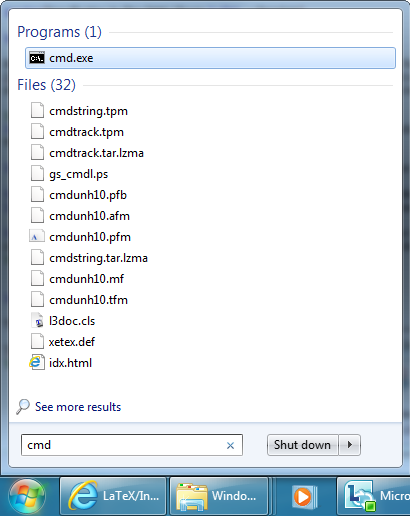
\includegraphics[scale=0.75]{TAMUthesis_CMD_windows.png}
\caption[Open CMD (Command Line Interface) under Windows]{Open CMD (Command Line Interface) under Windows
[Open the data/chapterI.tex file to search for the implementation of this figure, as you can
see that, to precisely contorl the position of the figure is not as straightforward as that in
Office Word.]}

\label{fig:CMD_1}

\end{figure}

\section{Figure Titles}

Some text here

\section{Continued Figures}
It's not recommended to use continued figures in this \LaTeX ~ document since figure/table numbering increases automatically. But if you would like to use it, refer to Figure \ref{fig:CMD_windows_cd_compile} for how Continued Figure works.

\begin{figure}[ht]
\centering
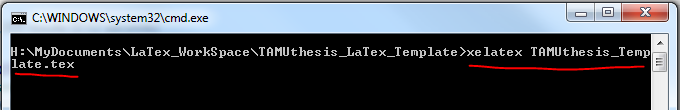
\includegraphics[scale=0.75]{TAMUthesis_CMD_windows_compile.png}
\caption{Compile .tex File}

\label{fig:CMD_windows_cd_compile}

\end{figure}
\cleardoublepage


\begin{figure}[ht]
\ContinuedFloat
\captionsetup{list=off, format=cont}
\centering
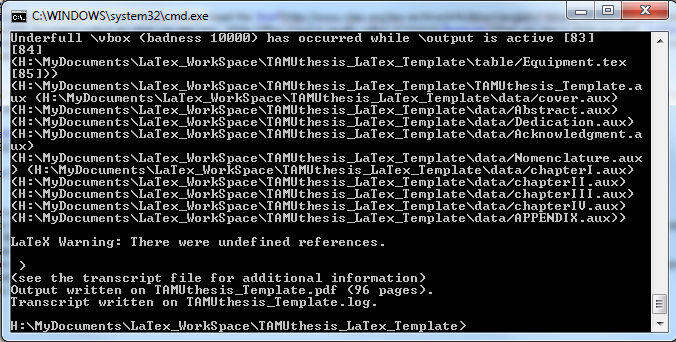
\includegraphics[scale=0.75]{TAMUthesis_CMD_windows_compile2.png}
\caption{[Example usage for Figure continued. Please don't display text for continued figures. This is just an example.]}

\label{fig:CMD_windows_cd_compile_continued}

\end{figure}


\section{Table Placement, Size and Table Title}


\begin{table}[!htbp]
\captionsetup{justification=centering}

\caption{Results from Experimental and Control Runs \label{table:control_runs}}

\begin{tabular}{|c|c|c|c|c|}
\hline
Species & Experiment 1 & Experiment 2 & Control 1 & Control 2\\
\hline
Cow & + & - & - & +\\
\hline
Brown Horse & - & + & - & -\\
\hline
Gray Cow &  &  &  & \\
\hline
White House & - & + & + & -\\
\hline
Tan Cow & + & - & - & +\\
\hline

\end{tabular}
\end{table}

 \cleardoublepage

 \begin{table}[!htbp]
 \ContinuedFloat
\captionsetup{list=off, format=cont}

 \label{table:control_runs_continued}
 
 \caption{} 

\begin{tabular}{|c|c|c|c|c|}
\hline
Species & Experiment 1 & Experiment 2 & Control 1 & Control 2\\
\hline
White Cow & + & - & - & +\\
\hline
Spotted Pig & + & + & + & -\\
\hline
White Pig & + & - & - & - \\
\hline
Brown Pig &  & + & + & -\\
\hline
Gray Pig & + & - & - & +\\
\hline
Black Pig & + & - & - & +\\
\hline

\end{tabular}
\end{table}



\section{Equations}

The following format is recommended to be used to display equations. The equation can be referred as Equ. \ref{Equ.2.1} and Equ. \ref{Equ.2.2}. 


\begin{equation} \label{Equ.2.1}
y'=y\cdot\cos{(a)}+x\cdot\sin{(a)}
\end{equation}

\begin{equation} \label{Equ.2.2}
e^{ja}=x\cdot\cos{(a)}-y\cdot\sin{(a)}
\end{equation}

Some sample equations are below


\begin{align}
V' &=e^{(ja)}\times V \label{Equ.3.3}\\
&=[\cos(a) + j \times \sin(a)] \times (x+j \times y) \label{Equ.3.4}\\
&=x \cdot \cos(a) - y\cdot \sin(a) + j \cdot [x \cdot \sin(a) + y \cdot     \cos(a)] \label{Equ.3.5}
\end{align}


\begin{equation}
\label{equ:matrix}
V=
\begin{bmatrix}
x'\\
y'\\
\end{bmatrix}=
\begin{bmatrix}
x \cdot \cos(a) - y \cdot \sin(a)\\
y \cdot \cos(a) + x \cdot \sin(a)\\
\end{bmatrix}
\end{equation}
Equ.\ref{equ:matrix} could be re-arranged as \ref{equ: 2.7} and  \ref{equ: 2.8}.

\begin{equation} 
\label{equ: 2.7}
x'=\cos(a) \cdot[x-y\cdot\tan(a)]
\end{equation}

\begin{equation} 
\label{equ: 2.8}
y'=\cos(a) \cdot [y+x \cdot \tan(a)]
\end{equation}



\begin{gather} 
x_{i+1}=\cos(a_i) \cdot [x_i-y_i \cdot 2^{-i} \cdot d_i] \label{Equ. 3.9}\\
y_{i+1}=\cos(a_i) \cdot [y_i+x_i \cdot 2^{-i} \cdot d_i] \label{Equ. 3.10}\\
\cos(\alpha)=\dfrac{1}{\sqrt [2]{1+{\tan(\alpha)}^2}}
 \label{Equ. 3.11} \\
K_i=\cos(\arctan(2^{-i}))= \dfrac{1}{\sqrt [2]{1+\tan(\arctan(2^{-   i}))}}=\dfrac{1}{\sqrt[2]{1+2^{-2i}}}
\label{Equ. 3.12}\\
\intertext{The product of $K_i$  represents the so-called $K$ factor (Equ. \ref{equ: 3.13})}
K=\prod K_i=\prod_{i=0}^{n-1} \dfrac{1}{\sqrt{1+2^{-2i}}}
\label{equ: 3.13}
\end{gather}


\section{Equation Vertical Spacing}

Test section for TOC display

\section{Other Information in this Document}
Test section for TOC display

\section{Another Test Section}
Test section for TOC display

\section{Another Test Section 3}
The section title is to test the toc only, no other purpose.

\section{Another Test Section 4}
Test section for TOC display

\section{Another Test Section 5 \& 6}
Test section for TOC display}







 





 

 
 


	\chapter{PROBLEM FORMULATION}
Consider a scenario where several wireless clients randomly located nearby a rectangular region. Four monitoring devices are located at the four corners. Each monitoring device has information of its own location and orientation. The radiation pattern of antenna attached to each monitoring device is known as well. All of the monitoring devices are connected to the Internet and send the captured data to a process center for inference. The wireless clients transmit data packets periodically and consequently detected by the monitoring devices. Since each wireless client has different MAC address, the packets transmitted from different clients can be distinguished. Here we use $\mathcal{A}_{\mathrm{t}}$ to represent the target area and $\mathcal{A}_{\mathrm{o}}$ to represent its complement.
In this study, we assume the wireless clients are quasi-static and each client is equipped with isotropic antenna. For convenience, we use a single vector to denote the locations of the wireless clients.
\begin{equation}
\underline{\mathbf{U}} = (\mathbf{U}_1, \ldots, \mathbf{U}_{n_{\mathrm{a}}}).
\end{equation}
where $n_{\mathrm{a}}$ is the number of the detected clients.
We also assume that the signal captured by a monitoring device comes from a line-of-sight path. Therefore the signal strength obeys free-space transmission model. The received signal strength from client $j$ to sensing device $i$ can be expressed as
\begin{equation} 
P_{ij} \text{[dBm]}
= A + B \log_{10}(d_{ij}) + L_{ij} + G_i (\phi_{ij})
\end{equation}
where $A$ and $B$ are the mean decay parameters, $d_{ij}$ is the Euclidean distance between the client $j$ and sensing device $i$. $L_{ij}$ is shadow fading parameter and $G_i (\cdot)$ is antenna gain function of sensing device. $\phi_{ij}$ is the angle of the signal transmission direction.
The shadow fading components $\{ L_{ij} \}$ are assumed to be independent and identically log-normal distributed random variables. In the logarithmic domain, the probability density function is
\begin{equation} 
f_{L_{ij}} (\ell)
= \frac{1}{\sqrt{2 \pi} \sigma_{\mathrm{s}}} 
\exp \left( - \frac{\ell^2}{2 \sigma_{\mathrm{s}}^2} \right)
\end{equation}
where $\sigma_{\mathrm{s}}$ is the standard deviation of shadowing.
The observed information from the four sensing devices form a power matrix $\underline{\mathbf{P}} = (\mathbf{P}_1, \ldots, \mathbf{P}_{n_{\mathrm{a}}})$. The vector element $\mathbf{P}_j = (P_{1j}, P_{2j},P_{3j},P_{4j})$ contains signal strength of wireless client j detected by four sensing devices.
We assume the number and locations of wireless clients located inside the area of interest form a Poisson point process with intensity $\lambda_{\mathrm{t}}$. Therefore
\begin{equation*}
\Pr ( R_{\mathrm{t}} = r_{\mathrm{t}} )
= \frac{(\lambda_{\mathrm{t}} A_{\mathrm{t}})^{r_{\mathrm{t}}}}
{r_{\mathrm{t}}!} e^{- A_{\mathrm{t}} \lambda_{\mathrm{t}}}
\quad r_{\mathrm{t}} = 0, 1, \ldots
\end{equation*}
Where $R_{\mathrm{t}}$ is the number of clients inside. $A_{\mathrm{t}}$ is the are of the target region.
Similarly, we get
\begin{equation*}
\Pr ( R_{\mathrm{o}} = r_{\mathrm{o}} )
= \frac{(\lambda_{\mathrm{o}} A_{\mathrm{o}})^{r_{\mathrm{o}}}}
{r_{\mathrm{o}}!} e^{- A_{\mathrm{o}} \lambda_{\mathrm{o}}}
\quad r_{\mathrm{o}} = 0, 1, \ldots
\end{equation*}
where $R_{\mathrm{o}}$ is the number of clients outside. $A_{\mathrm{o}}$ is the area of the complimentary of target region. $\lambda_{\mathrm{o}}$ is Poisson intensity parameter. The inference task is estimation the occupancy based on the Power matrix $\underline{\mathbf{P}}$.
\ignore{\section{Section Test Example 1 }


Test section for TOC display

\section{Test Section in this Chapter}

Section Title is to test toc display only, no actual meaning.

\subsection{Test Subsection in this Chapter}
Test subsection for TOC display

\subsection{Subsection Test Example 1}

Test subsection for TOC display

\section{Section Test Example 2}

Test section for TOC display

\subsection{Test Subsection in this Chapter}

Test subsection for TOC display

\subsection{Subsection Test Example 3 }
Test subsection for TOC display

Example of multiple line \textbf{verbatim} environment.

\begin{lstlisting}
  123
x 456
=============
  738 (this is 123 x 6)
 615  (this is 123 x 5, shifted one position to the left)
+492  (this is 123 x 4, shifted one position to the left)
=============
56088
\end{lstlisting}



\subsection*{Subsubsection Test Example 2}

some text here(the text will not be displayed in the TOC)


\subsection{Subsection Test Example 4}
Test subsection for TOC display

\subsection{Section Summary}
  
\begin{lstlisting}[language={Verilog},tabsize=5,title={A simple paragraph of Verilog code is below in verbatim}]
  Always@(posedge LRCK)
	Begin
	Counter = Counter + 1
	If (Counter == 40)
	Begin
	Counter = 0
	Phase_control_word = Phase_Control_word + 1
	If (phase_control_word >= 7168)
	Begin
	Phase_control_word =4778
	end
	end
	end
\end{lstlisting}

\section{Section Test Example 3}
Test section for toc display only

\subsection{Subsection Test 1}
Test subsection for toc display only.

\subsection{Subsection Test 2}
Test subsection for toc display only.

\subsection{Subsection Test 3}
Test subsection for toc display only.

\subsection{Subsection Test 4}
Test subsection for toc display only.

\section{Section Test Example 4}
Test section for toc display only}







	\chapter{ESTIMATION SCHEMES}

In this section, we introduce the two estimation schemes employed in this thesis.
A Bayes estimation scheme and a maximum likelihood estimation algorithm are considered and they are applied under different scenarios.
If the estimation process is applied repetitively over time, then acquired data can be employed to gain accurate estimates for $\lambda_{\mathrm{t}}$ and $\lambda_{\mathrm{o}}$.
In other words, $\lambda_{\mathrm{t}}$ and $\lambda_{\mathrm{o}}$ are considered known.
In such scenarios, Bayes estimation is employed.
On the other hand, if the occupancy estimation is applied to an area of interest once, then we can use a classic framework such as maximum likelihood estimation.


\section{Bayes Estimation} \label{section:BayesEstimation}

In the Bayes estimation scheme, we assume the Poisson intensity parameters $\lambda_{\mathrm{t}}$ and $\lambda_{\mathrm{o}}$ are known.
Our objective is to estimate the number of clients inside the target area based on observed data $\underline{\mathbf{P}}$.
First, we need to get the posterior distribution of $R_{\mathrm{t}}$, given $\underline{\mathbf{P}}$,
\begin{equation} \label{equation:PosdistRt}
\begin{split}
\Pr \left( R_{\mathrm{t}} = r_{\mathrm{t}}
| \underline{\mathbf{P}} = \underline{\mathbf{p}} \right)
&= \int_{ \left\{ \underline{\mathbf{u}}
	: R_{\mathrm{t}}(\underline{\mathbf{u}}) = r_{\mathrm{t}},
	R_{\mathrm{o}}(\underline{\mathbf{u}}) = r_{\mathrm{o}}
	\right\} }
f_{\underline{\mathbf{U}} | \underline{\mathbf{P}}}
\left( \underline{\mathbf{u}} | \underline{\mathbf{p}} \right)
d\underline{\mathbf{u}} \\
&= \int_{ \left\{ \underline{\mathbf{u}}
	: R_{\mathrm{t}}(\underline{\mathbf{u}}) = r_{\mathrm{t}},
	R_{\mathrm{o}}(\underline{\mathbf{u}}) = r_{\mathrm{o}} \right\} }
\frac{ f_{\underline{\mathbf{P}} | \underline{\mathbf{U}}}
	\left( \underline{\mathbf{p}} | \underline{\mathbf{u}} \right)
	f_{\underline{\mathbf{U}}} (\underline{\mathbf{u}}) }
{ f_{\underline{\mathbf{P}}} \left( \underline{\mathbf{p}} \right) }
d\underline{\mathbf{u}} 
\end{split}
\end{equation}
where $\underline{\mathbf{U}}$ is the location vector containing the random positions of the wireless clients. The location vector includes lots of information. For example, the size of $\underline{\mathbf{U}}$ is the number of active wireless clients.
According to the location vector, we can get the number of wireless clients inside or outside the target area.
Thus, $R_{t}$ and $R_{o}$ can be viewed as functions of $\underline{\mathbf{U}}$.
Because the outside and inside Poisson processes are independent, the distribution of $\underline{\mathbf{U}}$ can be written as
\begin{equation} \label{equation:distU}
\begin{split}
f_{\underline{\mathbf{U}}} ( \underline{\mathbf{u}} )
&= \frac{1}{A_{\mathrm{t}}^{R_{\mathrm{t}}(\underline{\mathbf{u}})}}
\frac{ ( \lambda_{\mathrm{t}}
	A_{\mathrm{t}} )^{R_{\mathrm{t}}(\underline{\mathbf{u}})} }
{ ( R_{\mathrm{t}}(\underline{\mathbf{u}}) )! }
e^{- A_{\mathrm{t}} \lambda_{\mathrm{t}}}
\frac{1}{A_{\mathrm{o}}^{R_{\mathrm{o}}(\underline{\mathbf{u}})}}
\frac{ ( \lambda_{\mathrm{o}}
	A_{\mathrm{o}} )^{R_{\mathrm{o}}(\underline{\mathbf{u}})} }
{ ( R_{\mathrm{o}}(\underline{\mathbf{u}}) )! }
e^{- A_{\mathrm{o}} \lambda_{\mathrm{o}}} \\
&= \frac{ \lambda_{\mathrm{t}}^{R_{\mathrm{t}}(\underline{\mathbf{u}})} }
{ ( R_{\mathrm{t}}(\underline{\mathbf{u}}) )! }
\frac{ \lambda_{\mathrm{o}}^{R_{\mathrm{o}}(\underline{\mathbf{u}})} }
{ ( R_{\mathrm{o}}(\underline{\mathbf{u}}) )! }
e^{- A_{\mathrm{t}} \lambda_{\mathrm{t}}
	- A_{\mathrm{o}} \lambda_{\mathrm{o}}} .
\end{split}
\end{equation}
For a wireless client $j$, the distribution of the received power vector $\mathbf{P}_j$ given a specific location $\mathbf{u}_j$ is equal to
\begin{equation} 
\begin{split}
f_{\mathbf{P}_j | \mathbf{U}_j} (\mathbf{p}_{j} | \mathbf{u}_j)
&= \prod_{i=1}^{n_{\mathrm{s}}}
f_{L_{ij}} ( p_{ij} - A - B \log_{10} (d_{ij}) - G_i(\phi_{ij}) ) \\
&= \frac{1}{\left( 2 \pi \sigma_{\mathrm{s}}^2 \right)^{\frac{n_{\mathrm{s}}}{2} }}
\prod_{i=1}^{n_{\mathrm{s}}} e^{- \frac{( p_{ij} - A - B \log_{10} (d_{ij}) - G_i(\phi_{ij}) )^2}{2 \sigma_{\mathrm{s}}^2} } \\
&= \left( 2 \pi \sigma_{\mathrm{s}}^2 \right)^{- \frac{n_{\mathrm{s}}}{2}}
e^{- \frac{ \sum_{i=1}^{n_{\mathrm{s}}}
(p_{ij} - A - B \log_{10} (d_{ij}) - G_i(\phi_{ij}))^2}
{2 \sigma_{\mathrm{s}}^2}} .
\end{split}
\end{equation}
The conditional distribution of $\underline{\mathbf{P}}$ given $\underline{\mathbf{U}}=\underline{\mathbf{u}}$, is then
\begin{equation} \label{equation:CondDistP}
f_{\underline{\mathbf{P}} | \underline{\mathbf{U}}}
\left( \underline{\mathbf{p}} | \underline{\mathbf{u}} \right)
= \prod_{j=1}^{n_{\mathrm{a}}}
f_{\mathbf{P}_j | \mathbf{U}_j} (\mathbf{p}_{j}|\mathbf{u}_j)  .
\end{equation}
With the conditional distribution of $\underline{\mathbf{P}}$ given $\underline{\mathbf{U}}=\underline{\mathbf{u}}$ and the distribution of $\underline{\mathbf{U}}$, we can compute the marginal distribution of $\underline{\mathbf{P}}$,
\begin{equation*}
\begin{split}
f_{\underline{\mathbf{P}}} \left( \underline{\mathbf{p}} \right)
&= \int_{ \left\{ \underline{\mathbf{u}}
	: R_{\mathrm{t}}(\underline{\mathbf{u}}) 
	+ R_{\mathrm{o}}(\underline{\mathbf{u}}) = n_{\mathrm{a}} \right\} }
f_{\underline{\mathbf{P}} | \underline{\mathbf{U}}}
\left( \underline{\mathbf{p}} | \underline{\mathbf{u}} \right)
f_{\underline{\mathbf{U}}}(\underline{\mathbf{u}})
d\underline{\mathbf{u}} \\
&= \sum_{(r_{\mathrm{t}}, r_{\mathrm{o}}) :
	r_{\mathrm{t}} + r_{\mathrm{o}} = n_{\mathrm{a}}}
\sum_{\{ \mathbb{I} \subset [n_{\mathrm{a}}]
	: |\mathbb{I}| = r_{\mathrm{t}} \}}
\frac{\lambda_{\mathrm{t}}^{r_{\mathrm{t}}}
	\lambda_{\mathrm{o}}^{r_{\mathrm{o}}}}
{r_{\mathrm{t}}! r_{\mathrm{o}}!}
e^{- A_{\mathrm{t}} \lambda_{\mathrm{t}}
	- A_{\mathrm{o}} \lambda_{\mathrm{o}}}
\prod_{j \in \mathbb{I}} \mathcal{I}_{\mathcal{A}_{\mathrm{t}}}(j)
\prod_{j \in \mathbb{I}^{\mathrm{c}}}
\mathcal{I}_{\mathcal{A}_{\mathrm{o}}}(j) ,
\end{split}
\end{equation*}
where the integral components are defined by
\begin{align} \label{equation:IntegralComponentsT}
\mathcal{I}_{\mathcal{A}_{\mathrm{t}}}(j)
&= \int_{\mathcal{A}_{\mathrm{t}}} f_{\mathbf{P}_j|\mathbf{U}_j}
(\mathbf{p}_j|\mathbf{u}_j) d\mathbf{u}_j \\
\label{equation:IntegralComponentsO}
\mathcal{I}_{\mathcal{A}_{\mathrm{o}}}(j)
&= \int_{\mathcal{A}_{\mathrm{o}}} f_{\mathbf{P}_j|\mathbf{U}_j}
(\mathbf{p}_j|\mathbf{u}_j) d\mathbf{u}_j .
\end{align}
Finally the posterior distribution of $R_{t}$, conditional on the gathered data is given by
\begin{equation*}
\begin{split}
	\Pr & \left( R_{\mathrm{t}} = r_{\mathrm{t}}
	| \underline{\mathbf{P}} = \underline{\mathbf{p}} \right) \\
	&= \sum_{\{ \mathbb{I} \subset [n_{\mathrm{a}}]
		: |\mathbb{I}| = r_{\mathrm{t}} \}}
	\frac{\lambda_{\mathrm{t}}^{r_{\mathrm{t}}}
		\lambda_{\mathrm{o}}^{r_{\mathrm{o}}}
		e^{- A_{\mathrm{t}} \lambda_{\mathrm{t}}
			- A_{\mathrm{o}} \lambda_{\mathrm{o}}}}
	{r_{\mathrm{t}}! r_{\mathrm{o}}!
		f_{\underline{\mathbf{P}}}(\underline{\mathbf{p}})}
	\prod_{j \in \mathbb{I}} \mathcal{I}_{\mathcal{A}_{\mathrm{t}}}(j)
	\prod_{j \in \mathbb{I}^{\mathrm{c}}} \mathcal{I}_{\mathcal{A}_{\mathrm{o}}}(j) .
\end{split}
\end{equation*}
Computing this conditional distribution of $R_{t}$ given $\underline{\mathbf{P}}$ may appear difficult as it entails taking sums over subsets of $\{ 1, \ldots, n_{\mathrm{a}} \}$.
However, by using generating functions, the posterior distribution can be calculated more efficiently~\cite{graham1994concrete}.

The mean of the posterior distribution of $R_{t}$ condition upon $\underline{\mathbf{P}}$ is the Bayes estimator,
\begin{equation} \label{equation:MMSE}
\hat{R}_{\mathrm{t}} \left( \underline{\mathbf{p}} \right)
= \mathrm{E} \left[ R_{\mathrm{t}}
| \underline{\mathbf{P}} = \underline{\mathbf{p}} \right]
= \sum_{r_{\mathrm{t}} = 0}^{n_{\mathrm{a}}} r_{\mathrm{t}}
\Pr \left( R_{\mathrm{t}} = r_{\mathrm{t}}
| \underline{\mathbf{P}} = \underline{\mathbf{p}} \right)  .
\end{equation}
We adopt the Bayesian mean squared error (BMSE) to evaluate the performance of the estimator,
\begin{equation} \label{equation:BMSE}
\mathrm{BMSE} \left[ \hat{R}_{\mathrm{t}} \right]
= \mathrm{E} \left[ \left(
\hat{R}_{\mathrm{t}} \left( \underline{\mathbf{P}} \right)
- R_{\mathrm{t}} \right)^2 \right] .
\end{equation}
This BMSE can be approximated by taking the average over samples,
\begin{equation} \label{equation:EmpiricalBMSE}
\mathrm{BMSE} \left[ \hat{R}_{\mathrm{t}} \right]
\approx \frac{1}{M} \sum_{m=1}^M \left(
\hat{R}_{\mathrm{t}}^{(m)} \left( \underline{\mathbf{P}}^{(m)} \right)
- R_{\mathrm{t}}^{(m)} \right)^2 .
\end{equation}


\section{Maximum likelihood estimation} \label{section:Maxestimation}

In this section, we assume the Poisson intensity parameters $\lambda_{\mathrm{t}}$ and $\lambda_{\mathrm{o}}$ are unavailable.
For this scenario, we employ a classical approach and adopt maximum-likelihood estimation~\cite{casella2001statistical}.
The distribution of $\underline{\mathbf{U}}$ can be written as
\begin{equation}
f_{\underline{\mathbf{U}}} \left( \underline{\mathbf{u}};
\lambda_{\mathrm{t}}, \lambda_{\mathrm{o}} \right)
= \frac{ \lambda_{\mathrm{t}}^{R_{\mathrm{t}}(\underline{\mathbf{u}})} }
{ ( R_{\mathrm{t}}(\underline{\mathbf{u}}) )! }
\frac{ \lambda_{\mathrm{o}}^{R_{\mathrm{o}}(\underline{\mathbf{u}})} }
{ ( R_{\mathrm{o}}(\underline{\mathbf{u}}) )! }
e^{- A_{\mathrm{t}} \lambda_{\mathrm{t}}
- A_{\mathrm{o}} \lambda_{\mathrm{o}}} .
\end{equation}
The likelihood function is a function with two parameters, $\lambda_{\mathrm{t}}$ and $\lambda_{\mathrm{o}}$
\begin{equation}
\mathcal{L} \left( \lambda_{\mathrm{t}}, \lambda_{\mathrm{o}};
\underline{\mathbf{p}}, \underline{\mathbf{u}} \right)
= f_{\underline{\mathbf{P}}, \underline{\mathbf{U}}}
\left( \underline{\mathbf{p}}, \underline{\mathbf{u}};
\lambda_{\mathrm{t}}, \lambda_{\mathrm{o}} \right)
= f_{\underline{\mathbf{P}} | \underline{\mathbf{U}}}
\left( \underline{\mathbf{p}} | \underline{\mathbf{u}} \right)
f_{\underline{\mathbf{U}}} \left( \underline{\mathbf{u}};
\lambda_{\mathrm{t}}, \lambda_{\mathrm{o}} \right) .
\end{equation}
By computing the integral over $\underline{\mathbf{U}}$, we can get the marginal likelihood function
\begin{equation} \label{equation:Likelihood}
\begin{split}
& \mathcal{L} \left( \lambda_{\mathrm{t}}, \lambda_{\mathrm{o}};
\underline{\mathbf{p}} \right)
= \int_{ \left\{ \underline{\mathbf{u}}
	: R_{\mathrm{t}}(\underline{\mathbf{u}}) +
	R_{\mathrm{o}}(\underline{\mathbf{u}}) = n_{\mathrm{a}} \right\} }
f_{\underline{\mathbf{P}} | \underline{\mathbf{U}}}
\left( \underline{\mathbf{p}} | \underline{\mathbf{u}} \right)
f_{\underline{\mathbf{U}}} \left( \underline{\mathbf{u}};
\lambda_{\mathrm{t}}, \lambda_{\mathrm{o}} \right) d\underline{\mathbf{u}} \\
&= e^{- A_{\mathrm{t}} \lambda_{\mathrm{t}}
	- A_{\mathrm{o}} \lambda_{\mathrm{o}}}
\sum_{(r_{\mathrm{t}}, r_{\mathrm{o}}) :
	r_{\mathrm{t}} + r_{\mathrm{o}} = n_{\mathrm{a}}}
\frac{\lambda_{\mathrm{t}}^{r_{\mathrm{t}}}
	\lambda_{\mathrm{o}}^{r_{\mathrm{o}}}}
{r_{\mathrm{t}}! r_{\mathrm{o}}!}
\sum_{\{ \mathbb{I} \subset [n_{\mathrm{a}}]
	: |\mathbb{I}| = r_{\mathrm{t}} \}}
\prod_{j \in \mathbb{I}}
\mathcal{I}_{\mathcal{A}_{\mathrm{t}}}(j)
\prod_{j \in \mathbb{I}^{\mathrm{c}}}
\mathcal{I}_{\mathcal{A}_{\mathrm{o}}}(j) .
\end{split}
\end{equation}
This results in a two-dimensional optimization for maximizing the likelihood.
But, we can simplify it to a one-dimensional optimization problem by the following property,
\begin{equation} 
\max_{\lambda_{\mathrm{t}}, \lambda_{\mathrm{o}}}
\mathcal{L} \left( \lambda_{\mathrm{t}}, \lambda_{\mathrm{o}};
\underline{\mathbf{p}} \right)
= \max_{\alpha} \mathcal{L} \left(
\frac{n_{\mathrm{a}}}{A_{\mathrm{t}}} \alpha ,
\frac{n_{\mathrm{a}}}{A_{\mathrm{o}}} (1 - \alpha) ;
\underline{\mathbf{p}} \right)
\end{equation}
where $\alpha$ within the interval $[0, 1]$.
Under this property, we can rewrite the likelihood function in terms of $\alpha$ as
\begin{equation}
\begin{split}
&\mathcal{L} \left(
\frac{n_{\mathrm{a}}}{A_{\mathrm{t}}} \alpha ,
\frac{n_{\mathrm{a}}}{A_{\mathrm{o}}} (1 - \alpha) ;
\underline{\mathbf{p}} \right) \\
&= \sum_{(r_{\mathrm{t}}, r_{\mathrm{o}}) :
	r_{\mathrm{t}} + r_{\mathrm{o}} = n_{\mathrm{a}}}
\frac{e^{- n_{\mathrm{a}}} n_{\mathrm{a}}^{n_{\mathrm{a}}}}
{r_{\mathrm{t}}! r_{\mathrm{o}}!}
\left( \frac{\alpha}{A_{\mathrm{t}}} \right)^{r_{\mathrm{t}}}
\left( \frac{1 - \alpha}{A_{\mathrm{o}}} \right)^{r_{\mathrm{o}}}
\sum_{\{ \mathbb{I} \subset [n_{\mathrm{a}}] : |\mathbb{I}| = r_{\mathrm{t}} \}}
\prod_{j \in \mathbb{I}} \mathcal{I}_{\mathcal{A}_{\mathrm{t}}}(j)
\prod_{j \in \mathbb{I}^{\mathrm{c}}}
\mathcal{I}_{\mathcal{A}_{\mathrm{o}}}(j) .
\end{split}
\end{equation}
At this point, we can use standard numerical methods to get the values of $\lambda_{\mathrm{t}}$ and $\lambda_{\mathrm{o}}$ that maximize the likelihood function.
Once $\lambda_{\mathrm{t}}$ and $\lambda_{\mathrm{o}}$ are obtained, the maximum likelihood estimator can be calculated as
\begin{equation} 
\begin{split}
\hat{R}_{\mathrm{t}}
\left( \underline{\mathbf{p}} \right)
&= \mathrm{E}_{\hat{\lambda}_{\mathrm{t}}, \hat{\lambda}_{\mathrm{o}}}
\left[ R_{\mathrm{t}} | \underline{\mathbf{P}}
= \underline{\mathbf{p}} \right] \\
&= \sum_{r_{\mathrm{t}} = 0}^{n_{\mathrm{a}}} r_{\mathrm{t}}
\Pr \left( R_{\mathrm{t}} = r_{\mathrm{t}}
| \underline{\mathbf{P}} = \underline{\mathbf{p}} ;
\hat{\lambda}_{\mathrm{t}}, \hat{\lambda}_{\mathrm{o}} \right) .
\end{split}
\end{equation}
We adopt the mean squared error (MSE) to evaluate the performance of our estimator,
\begin{equation} \label{equation:MSE}
\mathrm{MSE} \left[ \hat{R}_{\mathrm{t}} \right]
= \mathrm{E} \left[ \left(
\hat{R}_{\mathrm{t}} \left( \underline{\mathbf{P}} \right)
- R_{\mathrm{t}} \right)^2 \right] .
\end{equation}
This mean squared error can be approximated by taking the average over samples numerically,
\begin{equation} \label{equation:EmpiricalMSE}
\mathrm{MSE} \left[ \hat{R}_{\mathrm{t}} \right]
\approx \frac{1}{M} \sum_{m=1}^M \left(
\hat{R}_{\mathrm{t}}^{(m)} \left( \underline{\mathbf{P}}^{(m)} \right)
- R_{\mathrm{t}}^{(m)} \right)^2  .
\end{equation}



	\chapter{NUMERICAL SIMULATION SETUP AND RESULTS}

In this section, we introduce our simulation setup, including the directional antenna model, the parameters of the channel and how we generate RSSI samples.
The simulation results will be shown after that.
The simulation code is written in Python.
In the simulation framework, the set up consists of four monitoring devices placed at the corners of the area of interest.
All antennas attached to monitoring devices are pointing towards the center of the area of interest.
The target area is considered to be a square of dimension 6~m~×~6~m inscribed in a larger square of dimension 10~m×10~m.
The two square areas share a same center point.
Again, we use $A_{t}$ to denote the target area, while $A_{o}$ denotes its complement.
We call the inside region the target area, and we refer to its complement as the outside region in the following text.


\section{Antenna Characteristic}

To analyze the effect of radiation characteristics of the sensing antennas on the estimation, isotropic antennas and directional antennas are considered.
The antenna gain of the isotropic antennas are zero in all directions.
For the directional antennas, we adopt the 3GPP antenna model in~\cite{3GPP-antenna}.
The directional antenna gains obey the following formula,
\begin{equation*}
G_i (\phi_{ij}) = - \min \left\{
12 \left( \frac{\phi_{ij} - \theta_{i}}{\theta_{\mathrm{3dB}}} \right)^2,
G_{\mathrm{floor}} \right\} - G_{\mathrm{avg}}
\end{equation*}
where $\theta_{i}$ is the pointing direction of the antenna that is attached to monitoring device~$i$.
Parameter $\theta_{\mathrm{3dB}}$ is the 3~dB beam-width of the radiation pattern.
Variable $G_{floor}$ is a nominal attenuation floor.
And, $G_{average}$ is a normalization factor, which equal to the average gain over $\in (-180^{\circ}, 180^{\circ}]$,
\begin{equation*}
10 \log_{10} \left( \int_{-180}^{180}
\frac{ 10^{ - \frac{1}{10} \min \left\{
12 \left( \frac{\phi_{ij} - \theta_{i}}{\theta_{\mathrm{3dB}}} \right)^2,
G_{\mathrm{floor}} \right\} } }{360} d \phi_{ij} \right) .
\end{equation*}
The antenna radiation pattern for various 3~dB beam-widths is shown in Fig.~\ref{figure:AntennaCandidates}.
\begin{figure}[t]
	\centerline{\begin{tikzpicture}
\begin{polaraxis}[
%scale only axis,
width=7cm,
xticklabel=$\pgfmathprintnumber{\tick}^\circ$,
y coord trafo/.code=\pgfmathparse{#1+20},
ytick={-16, -8, 0, 8},
ymin=-18, ymax=12,
y coord inv trafo/.code=\pgfmathparse{#1-20},
%height=5cm,
%xlabel={Angle (degree)},
%ylabel={Gain (dB)},
every tick label/.append style={font=\small},
legend entries={\scriptsize{Isotropic},
\scriptsize{$\theta_{\mathrm{3dB}} = 30^{\circ}$},
\scriptsize{$\theta_{\mathrm{3dB}} = 60^{\circ}$},
\scriptsize{$\theta_{\mathrm{3dB}} = 90^{\circ}$},
\scriptsize{$\theta_{\mathrm{3dB}} = 120^{\circ}$}},
legend style={at={(-0.1,0.15)}, nodes=right}
]

% Isotropic
\addplot [
color=black,
densely dotted,
line width=1.5pt
]
coordinates{
(-180, 0) (-179, 0) (-178, 0) (-177, 0)
(-176, 0) (-175, 0) (-174, 0) (-173, 0)
(-172, 0) (-171, 0) (-170, 0) (-169, 0)
(-168, 0) (-167, 0) (-166, 0) (-165, 0)
(-164, 0) (-163, 0) (-162, 0) (-161, 0)
(-160, 0) (-159, 0) (-158, 0) (-157, 0)
(-156, 0) (-155, 0) (-154, 0) (-153, 0)
(-152, 0) (-151, 0) (-150, 0) (-149, 0)
(-148, 0) (-147, 0) (-146, 0) (-145, 0)
(-144, 0) (-143, 0) (-142, 0) (-141, 0)
(-140, 0) (-139, 0) (-138, 0) (-137, 0)
(-136, 0) (-135, 0) (-134, 0) (-133, 0)
(-132, 0) (-131, 0) (-130, 0) (-129, 0)
(-128, 0) (-127, 0) (-126, 0) (-125, 0)
(-124, 0) (-123, 0) (-122, 0) (-121, 0)
(-120, 0) (-119, 0) (-118, 0) (-117, 0)
(-116, 0) (-115, 0) (-114, 0) (-113, 0)
(-112, 0) (-111, 0) (-110, 0) (-109, 0)
(-108, 0) (-107, 0) (-106, 0) (-105, 0)
(-104, 0) (-103, 0) (-102, 0) (-101, 0)
(-100, 0) (-99, 0) (-98, 0) (-97, 0)
(-96, 0) (-95, 0) (-94, 0) (-93, 0)
(-92, 0) (-91, 0) (-90, 0) (-89, 0)
(-88, 0) (-87, 0) (-86, 0) (-85, 0)
(-84, 0) (-83, 0) (-82, 0) (-81, 0)
(-80, 0) (-79, 0) (-78, 0) (-77, 0)
(-76, 0) (-75, 0) (-74, 0) (-73, 0)
(-72, 0) (-71, 0) (-70, 0) (-69, 0)
(-68, 0) (-67, 0) (-66, 0) (-65, 0)
(-64, 0) (-63, 0) (-62, 0) (-61, 0)
(-60, 0) (-59, 0) (-58, 0) (-57, 0)
(-56, 0) (-55, 0) (-54, 0) (-53, 0)
(-52, 0) (-51, 0) (-50, 0) (-49, 0)
(-48, 0) (-47, 0) (-46, 0) (-45, 0)
(-44, 0) (-43, 0) (-42, 0) (-41, 0)
(-40, 0) (-39, 0) (-38, 0) (-37, 0)
(-36, 0) (-35, 0) (-34, 0) (-33, 0)
(-32, 0) (-31, 0) (-30, 0) (-29, 0)
(-28, 0) (-27, 0) (-26, 0) (-25, 0)
(-24, 0) (-23, 0) (-22, 0) (-21, 0)
(-20, 0) (-19, 0) (-18, 0) (-17, 0)
(-16, 0) (-15, 0) (-14, 0) (-13, 0)
(-12, 0) (-11, 0) (-10, 0) ( -9, 0)
( -8, 0) ( -7, 0) ( -6, 0) ( -5, 0)
( -4, 0) ( -3, 0) ( -2, 0) ( -1, 0)
(  0, 0) (  1, 0) (  2, 0) (  3, 0)
(  4, 0) (  5, 0) (  6, 0) (  7, 0)
(  8, 0) (  9, 0) ( 10, 0) ( 11, 0)
( 12, 0) ( 13, 0) ( 14, 0) ( 15, 0)
( 16, 0) ( 17, 0) ( 18, 0) ( 19, 0)
( 20, 0) ( 21, 0) ( 22, 0) ( 23, 0)
( 24, 0) ( 25, 0) ( 26, 0) ( 27, 0)
( 28, 0) ( 29, 0) ( 30, 0) ( 31, 0)
( 32, 0) ( 33, 0) ( 34, 0) ( 35, 0)
( 36, 0) ( 37, 0) ( 38, 0) ( 39, 0)
( 40, 0) ( 41, 0) ( 42, 0) ( 43, 0)
( 44, 0) ( 45, 0) ( 46, 0) ( 47, 0)
( 48, 0) ( 49, 0) ( 50, 0) ( 51, 0)
( 52, 0) ( 53, 0) ( 54, 0) ( 55, 0)
( 56, 0) ( 57, 0) ( 58, 0) ( 59, 0)
( 60, 0) ( 61, 0) ( 62, 0) ( 63, 0)
( 64, 0) ( 65, 0) ( 66, 0) ( 67, 0)
( 68, 0) ( 69, 0) ( 70, 0) ( 71, 0)
( 72, 0) ( 73, 0) ( 74, 0) ( 75, 0)
( 76, 0) ( 77, 0) ( 78, 0) ( 79, 0)
( 80, 0) ( 81, 0) ( 82, 0) ( 83, 0)
( 84, 0) ( 85, 0) ( 86, 0) ( 87, 0)
( 88, 0) ( 89, 0) ( 90, 0) ( 91, 0)
( 92, 0) ( 93, 0) ( 94, 0) ( 95, 0)
( 96, 0) ( 97, 0) ( 98, 0) ( 99, 0)
(100, 0) (101, 0) (102, 0) (103, 0)
(104, 0) (105, 0) (106, 0) (107, 0)
(108, 0) (109, 0) (110, 0) (111, 0)
(112, 0) (113, 0) (114, 0) (115, 0)
(116, 0) (117, 0) (118, 0) (119, 0)
(120, 0) (121, 0) (122, 0) (123, 0)
(124, 0) (125, 0) (126, 0) (127, 0)
(128, 0) (129, 0) (130, 0) (131, 0)
(132, 0) (133, 0) (134, 0) (135, 0)
(136, 0) (137, 0) (138, 0) (139, 0)
(140, 0) (141, 0) (142, 0) (143, 0)
(144, 0) (145, 0) (146, 0) (147, 0)
(148, 0) (149, 0) (150, 0) (151, 0)
(152, 0) (153, 0) (154, 0) (155, 0)
(156, 0) (157, 0) (158, 0) (159, 0)
(160, 0) (161, 0) (162, 0) (163, 0)
(164, 0) (165, 0) (166, 0) (167, 0)
(168, 0) (169, 0) (170, 0) (171, 0)
(172, 0) (173, 0) (174, 0) (175, 0)
(176, 0) (177, 0) (178, 0) (179, 0)
(180, 0)
};

% Theta3dB = 30.0
\addplot [
color=gray,
densely dashed,
line width=1.0pt
]
coordinates{
(-180, -9.8341) (-179, -9.8341) (-178, -9.8341) (-177, -9.8341)
(-176, -9.8341) (-175, -9.8341) (-174, -9.8341) (-173, -9.8341)
(-172, -9.8341) (-171, -9.8341) (-170, -9.8341) (-169, -9.8341)
(-168, -9.8341) (-167, -9.8341) (-166, -9.8341) (-165, -9.8341)
(-164, -9.8341) (-163, -9.8341) (-162, -9.8341) (-161, -9.8341)
(-160, -9.8341) (-159, -9.8341) (-158, -9.8341) (-157, -9.8341)
(-156, -9.8341) (-155, -9.8341) (-154, -9.8341) (-153, -9.8341)
(-152, -9.8341) (-151, -9.8341) (-150, -9.8341) (-149, -9.8341)
(-148, -9.8341) (-147, -9.8341) (-146, -9.8341) (-145, -9.8341)
(-144, -9.8341) (-143, -9.8341) (-142, -9.8341) (-141, -9.8341)
(-140, -9.8341) (-139, -9.8341) (-138, -9.8341) (-137, -9.8341)
(-136, -9.8341) (-135, -9.8341) (-134, -9.8341) (-133, -9.8341)
(-132, -9.8341) (-131, -9.8341) (-130, -9.8341) (-129, -9.8341)
(-128, -9.8341) (-127, -9.8341) (-126, -9.8341) (-125, -9.8341)
(-124, -9.8341) (-123, -9.8341) (-122, -9.8341) (-121, -9.8341)
(-120, -9.8341) (-119, -9.8341) (-118, -9.8341) (-117, -9.8341)
(-116, -9.8341) (-115, -9.8341) (-114, -9.8341) (-113, -9.8341)
(-112, -9.8341) (-111, -9.8341) (-110, -9.8341) (-109, -9.8341)
(-108, -9.8341) (-107, -9.8341) (-106, -9.8341) (-105, -9.8341)
(-104, -9.8341) (-103, -9.8341) (-102, -9.8341) (-101, -9.8341)
(-100, -9.8341) (-99, -9.8341) (-98, -9.8341) (-97, -9.8341)
(-96, -9.8341) (-95, -9.8341) (-94, -9.8341) (-93, -9.8341)
(-92, -9.8341) (-91, -9.8341) (-90, -9.8341) (-89, -9.8341)
(-88, -9.8341) (-87, -9.8341) (-86, -9.8341) (-85, -9.8341)
(-84, -9.8341) (-83, -9.8341) (-82, -9.8341) (-81, -9.8341)
(-80, -9.8341) (-79, -9.8341) (-78, -9.8341) (-77, -9.8341)
(-76, -9.8341) (-75, -9.8341) (-74, -9.8341) (-73, -9.8341)
(-72, -9.8341) (-71, -9.8341) (-70, -9.8341) (-69, -9.8341)
(-68, -9.8341) (-67, -9.8341) (-66, -9.8341) (-65, -9.8341)
(-64, -9.8341) (-63, -9.8341) (-62, -9.8341) (-61, -9.8341)
(-60, -9.8341) (-59, -9.8341) (-58, -9.8341) (-57, -9.8341)
(-56, -9.8341) (-55, -9.8341) (-54, -9.8341) (-53, -9.8341)
(-52, -9.8341) (-51, -9.8341) (-50, -9.8341) (-49, -9.8341)
(-48, -9.8341) (-47, -9.8341) (-46, -9.8341) (-45, -9.8341)
(-44, -9.8341) (-43, -9.8341) (-42, -9.8341) (-41, -9.8341)
(-40, -9.8341) (-39, -9.8341) (-38, -9.0875) (-37, -8.0875)
(-36, -7.1141) (-35, -6.1675) (-34, -5.2475) (-33, -4.3541)
(-32, -3.4875) (-31, -2.6475) (-30, -1.8341) (-29, -1.0475)
(-28, -0.2875) (-27, 0.4459) (-26, 1.1525) (-25, 1.8325)
(-24, 2.4859) (-23, 3.1125) (-22, 3.7125) (-21, 4.2859)
(-20, 4.8325) (-19, 5.3525) (-18, 5.8459) (-17, 6.3125)
(-16, 6.7525) (-15, 7.1659) (-14, 7.5525) (-13, 7.9125)
(-12, 8.2459) (-11, 8.5525) (-10, 8.8325) ( -9, 9.0859)
( -8, 9.3125) ( -7, 9.5125) ( -6, 9.6859) ( -5, 9.8325)
( -4, 9.9525) ( -3, 10.0459) ( -2, 10.1125) ( -1, 10.1525)
(  0, 10.1659) (  1, 10.1525) (  2, 10.1125) (  3, 10.0459)
(  4, 9.9525) (  5, 9.8325) (  6, 9.6859) (  7, 9.5125)
(  8, 9.3125) (  9, 9.0859) ( 10, 8.8325) ( 11, 8.5525)
( 12, 8.2459) ( 13, 7.9125) ( 14, 7.5525) ( 15, 7.1659)
( 16, 6.7525) ( 17, 6.3125) ( 18, 5.8459) ( 19, 5.3525)
( 20, 4.8325) ( 21, 4.2859) ( 22, 3.7125) ( 23, 3.1125)
( 24, 2.4859) ( 25, 1.8325) ( 26, 1.1525) ( 27, 0.4459)
( 28, -0.2875) ( 29, -1.0475) ( 30, -1.8341) ( 31, -2.6475)
( 32, -3.4875) ( 33, -4.3541) ( 34, -5.2475) ( 35, -6.1675)
( 36, -7.1141) ( 37, -8.0875) ( 38, -9.0875) ( 39, -9.8341)
( 40, -9.8341) ( 41, -9.8341) ( 42, -9.8341) ( 43, -9.8341)
( 44, -9.8341) ( 45, -9.8341) ( 46, -9.8341) ( 47, -9.8341)
( 48, -9.8341) ( 49, -9.8341) ( 50, -9.8341) ( 51, -9.8341)
( 52, -9.8341) ( 53, -9.8341) ( 54, -9.8341) ( 55, -9.8341)
( 56, -9.8341) ( 57, -9.8341) ( 58, -9.8341) ( 59, -9.8341)
( 60, -9.8341) ( 61, -9.8341) ( 62, -9.8341) ( 63, -9.8341)
( 64, -9.8341) ( 65, -9.8341) ( 66, -9.8341) ( 67, -9.8341)
( 68, -9.8341) ( 69, -9.8341) ( 70, -9.8341) ( 71, -9.8341)
( 72, -9.8341) ( 73, -9.8341) ( 74, -9.8341) ( 75, -9.8341)
( 76, -9.8341) ( 77, -9.8341) ( 78, -9.8341) ( 79, -9.8341)
( 80, -9.8341) ( 81, -9.8341) ( 82, -9.8341) ( 83, -9.8341)
( 84, -9.8341) ( 85, -9.8341) ( 86, -9.8341) ( 87, -9.8341)
( 88, -9.8341) ( 89, -9.8341) ( 90, -9.8341) ( 91, -9.8341)
( 92, -9.8341) ( 93, -9.8341) ( 94, -9.8341) ( 95, -9.8341)
( 96, -9.8341) ( 97, -9.8341) ( 98, -9.8341) ( 99, -9.8341)
(100, -9.8341) (101, -9.8341) (102, -9.8341) (103, -9.8341)
(104, -9.8341) (105, -9.8341) (106, -9.8341) (107, -9.8341)
(108, -9.8341) (109, -9.8341) (110, -9.8341) (111, -9.8341)
(112, -9.8341) (113, -9.8341) (114, -9.8341) (115, -9.8341)
(116, -9.8341) (117, -9.8341) (118, -9.8341) (119, -9.8341)
(120, -9.8341) (121, -9.8341) (122, -9.8341) (123, -9.8341)
(124, -9.8341) (125, -9.8341) (126, -9.8341) (127, -9.8341)
(128, -9.8341) (129, -9.8341) (130, -9.8341) (131, -9.8341)
(132, -9.8341) (133, -9.8341) (134, -9.8341) (135, -9.8341)
(136, -9.8341) (137, -9.8341) (138, -9.8341) (139, -9.8341)
(140, -9.8341) (141, -9.8341) (142, -9.8341) (143, -9.8341)
(144, -9.8341) (145, -9.8341) (146, -9.8341) (147, -9.8341)
(148, -9.8341) (149, -9.8341) (150, -9.8341) (151, -9.8341)
(152, -9.8341) (153, -9.8341) (154, -9.8341) (155, -9.8341)
(156, -9.8341) (157, -9.8341) (158, -9.8341) (159, -9.8341)
(160, -9.8341) (161, -9.8341) (162, -9.8341) (163, -9.8341)
(164, -9.8341) (165, -9.8341) (166, -9.8341) (167, -9.8341)
(168, -9.8341) (169, -9.8341) (170, -9.8341) (171, -9.8341)
(172, -9.8341) (173, -9.8341) (174, -9.8341) (175, -9.8341)
(176, -9.8341) (177, -9.8341) (178, -9.8341) (179, -9.8341)
(180, -9.8341)
};

% Theta3dB = 60.0
\addplot [
color=gray,
dashed,
line width=1.0pt
]
coordinates{
(-180, -12.6128) (-179, -12.6128) (-178, -12.6128) (-177, -12.6128)
(-176, -12.6128) (-175, -12.6128) (-174, -12.6128) (-173, -12.6128)
(-172, -12.6128) (-171, -12.6128) (-170, -12.6128) (-169, -12.6128)
(-168, -12.6128) (-167, -12.6128) (-166, -12.6128) (-165, -12.6128)
(-164, -12.6128) (-163, -12.6128) (-162, -12.6128) (-161, -12.6128)
(-160, -12.6128) (-159, -12.6128) (-158, -12.6128) (-157, -12.6128)
(-156, -12.6128) (-155, -12.6128) (-154, -12.6128) (-153, -12.6128)
(-152, -12.6128) (-151, -12.6128) (-150, -12.6128) (-149, -12.6128)
(-148, -12.6128) (-147, -12.6128) (-146, -12.6128) (-145, -12.6128)
(-144, -12.6128) (-143, -12.6128) (-142, -12.6128) (-141, -12.6128)
(-140, -12.6128) (-139, -12.6128) (-138, -12.6128) (-137, -12.6128)
(-136, -12.6128) (-135, -12.6128) (-134, -12.6128) (-133, -12.6128)
(-132, -12.6128) (-131, -12.6128) (-130, -12.6128) (-129, -12.6128)
(-128, -12.6128) (-127, -12.6128) (-126, -12.6128) (-125, -12.6128)
(-124, -12.6128) (-123, -12.6128) (-122, -12.6128) (-121, -12.6128)
(-120, -12.6128) (-119, -12.6128) (-118, -12.6128) (-117, -12.6128)
(-116, -12.6128) (-115, -12.6128) (-114, -12.6128) (-113, -12.6128)
(-112, -12.6128) (-111, -12.6128) (-110, -12.6128) (-109, -12.6128)
(-108, -12.6128) (-107, -12.6128) (-106, -12.6128) (-105, -12.6128)
(-104, -12.6128) (-103, -12.6128) (-102, -12.6128) (-101, -12.6128)
(-100, -12.6128) (-99, -12.6128) (-98, -12.6128) (-97, -12.6128)
(-96, -12.6128) (-95, -12.6128) (-94, -12.6128) (-93, -12.6128)
(-92, -12.6128) (-91, -12.6128) (-90, -12.6128) (-89, -12.6128)
(-88, -12.6128) (-87, -12.6128) (-86, -12.6128) (-85, -12.6128)
(-84, -12.6128) (-83, -12.6128) (-82, -12.6128) (-81, -12.6128)
(-80, -12.6128) (-79, -12.6128) (-78, -12.6128) (-77, -12.3761)
(-76, -11.8661) (-75, -11.3628) (-74, -10.8661) (-73, -10.3761)
(-72, -9.8928) (-71, -9.4161) (-70, -8.9461) (-69, -8.4828)
(-68, -8.0261) (-67, -7.5761) (-66, -7.1328) (-65, -6.6961)
(-64, -6.2661) (-63, -5.8428) (-62, -5.4261) (-61, -5.0161)
(-60, -4.6128) (-59, -4.2161) (-58, -3.8261) (-57, -3.4428)
(-56, -3.0661) (-55, -2.6961) (-54, -2.3328) (-53, -1.9761)
(-52, -1.6261) (-51, -1.2828) (-50, -0.9461) (-49, -0.6161)
(-48, -0.2928) (-47, 0.0239) (-46, 0.3339) (-45, 0.6372)
(-44, 0.9339) (-43, 1.2239) (-42, 1.5072) (-41, 1.7839)
(-40, 2.0539) (-39, 2.3172) (-38, 2.5739) (-37, 2.8239)
(-36, 3.0672) (-35, 3.3039) (-34, 3.5339) (-33, 3.7572)
(-32, 3.9739) (-31, 4.1839) (-30, 4.3872) (-29, 4.5839)
(-28, 4.7739) (-27, 4.9572) (-26, 5.1339) (-25, 5.3039)
(-24, 5.4672) (-23, 5.6239) (-22, 5.7739) (-21, 5.9172)
(-20, 6.0539) (-19, 6.1839) (-18, 6.3072) (-17, 6.4239)
(-16, 6.5339) (-15, 6.6372) (-14, 6.7339) (-13, 6.8239)
(-12, 6.9072) (-11, 6.9839) (-10, 7.0539) ( -9, 7.1172)
( -8, 7.1739) ( -7, 7.2239) ( -6, 7.2672) ( -5, 7.3039)
( -4, 7.3339) ( -3, 7.3572) ( -2, 7.3739) ( -1, 7.3839)
(  0, 7.3872) (  1, 7.3839) (  2, 7.3739) (  3, 7.3572)
(  4, 7.3339) (  5, 7.3039) (  6, 7.2672) (  7, 7.2239)
(  8, 7.1739) (  9, 7.1172) ( 10, 7.0539) ( 11, 6.9839)
( 12, 6.9072) ( 13, 6.8239) ( 14, 6.7339) ( 15, 6.6372)
( 16, 6.5339) ( 17, 6.4239) ( 18, 6.3072) ( 19, 6.1839)
( 20, 6.0539) ( 21, 5.9172) ( 22, 5.7739) ( 23, 5.6239)
( 24, 5.4672) ( 25, 5.3039) ( 26, 5.1339) ( 27, 4.9572)
( 28, 4.7739) ( 29, 4.5839) ( 30, 4.3872) ( 31, 4.1839)
( 32, 3.9739) ( 33, 3.7572) ( 34, 3.5339) ( 35, 3.3039)
( 36, 3.0672) ( 37, 2.8239) ( 38, 2.5739) ( 39, 2.3172)
( 40, 2.0539) ( 41, 1.7839) ( 42, 1.5072) ( 43, 1.2239)
( 44, 0.9339) ( 45, 0.6372) ( 46, 0.3339) ( 47, 0.0239)
( 48, -0.2928) ( 49, -0.6161) ( 50, -0.9461) ( 51, -1.2828)
( 52, -1.6261) ( 53, -1.9761) ( 54, -2.3328) ( 55, -2.6961)
( 56, -3.0661) ( 57, -3.4428) ( 58, -3.8261) ( 59, -4.2161)
( 60, -4.6128) ( 61, -5.0161) ( 62, -5.4261) ( 63, -5.8428)
( 64, -6.2661) ( 65, -6.6961) ( 66, -7.1328) ( 67, -7.5761)
( 68, -8.0261) ( 69, -8.4828) ( 70, -8.9461) ( 71, -9.4161)
( 72, -9.8928) ( 73, -10.3761) ( 74, -10.8661) ( 75, -11.3628)
( 76, -11.8661) ( 77, -12.3761) ( 78, -12.6128) ( 79, -12.6128)
( 80, -12.6128) ( 81, -12.6128) ( 82, -12.6128) ( 83, -12.6128)
( 84, -12.6128) ( 85, -12.6128) ( 86, -12.6128) ( 87, -12.6128)
( 88, -12.6128) ( 89, -12.6128) ( 90, -12.6128) ( 91, -12.6128)
( 92, -12.6128) ( 93, -12.6128) ( 94, -12.6128) ( 95, -12.6128)
( 96, -12.6128) ( 97, -12.6128) ( 98, -12.6128) ( 99, -12.6128)
(100, -12.6128) (101, -12.6128) (102, -12.6128) (103, -12.6128)
(104, -12.6128) (105, -12.6128) (106, -12.6128) (107, -12.6128)
(108, -12.6128) (109, -12.6128) (110, -12.6128) (111, -12.6128)
(112, -12.6128) (113, -12.6128) (114, -12.6128) (115, -12.6128)
(116, -12.6128) (117, -12.6128) (118, -12.6128) (119, -12.6128)
(120, -12.6128) (121, -12.6128) (122, -12.6128) (123, -12.6128)
(124, -12.6128) (125, -12.6128) (126, -12.6128) (127, -12.6128)
(128, -12.6128) (129, -12.6128) (130, -12.6128) (131, -12.6128)
(132, -12.6128) (133, -12.6128) (134, -12.6128) (135, -12.6128)
(136, -12.6128) (137, -12.6128) (138, -12.6128) (139, -12.6128)
(140, -12.6128) (141, -12.6128) (142, -12.6128) (143, -12.6128)
(144, -12.6128) (145, -12.6128) (146, -12.6128) (147, -12.6128)
(148, -12.6128) (149, -12.6128) (150, -12.6128) (151, -12.6128)
(152, -12.6128) (153, -12.6128) (154, -12.6128) (155, -12.6128)
(156, -12.6128) (157, -12.6128) (158, -12.6128) (159, -12.6128)
(160, -12.6128) (161, -12.6128) (162, -12.6128) (163, -12.6128)
(164, -12.6128) (165, -12.6128) (166, -12.6128) (167, -12.6128)
(168, -12.6128) (169, -12.6128) (170, -12.6128) (171, -12.6128)
(172, -12.6128) (173, -12.6128) (174, -12.6128) (175, -12.6128)
(176, -12.6128) (177, -12.6128) (178, -12.6128) (179, -12.6128)
(180, -12.6128)
};

% Theta3dB = 90.0
\addplot [
color=black,
solid,
line width=1.5pt
]
coordinates{
(-180, -14.2936) (-179, -14.2936) (-178, -14.2936) (-177, -14.2936)
(-176, -14.2936) (-175, -14.2936) (-174, -14.2936) (-173, -14.2936)
(-172, -14.2936) (-171, -14.2936) (-170, -14.2936) (-169, -14.2936)
(-168, -14.2936) (-167, -14.2936) (-166, -14.2936) (-165, -14.2936)
(-164, -14.2936) (-163, -14.2936) (-162, -14.2936) (-161, -14.2936)
(-160, -14.2936) (-159, -14.2936) (-158, -14.2936) (-157, -14.2936)
(-156, -14.2936) (-155, -14.2936) (-154, -14.2936) (-153, -14.2936)
(-152, -14.2936) (-151, -14.2936) (-150, -14.2936) (-149, -14.2936)
(-148, -14.2936) (-147, -14.2936) (-146, -14.2936) (-145, -14.2936)
(-144, -14.2936) (-143, -14.2936) (-142, -14.2936) (-141, -14.2936)
(-140, -14.2936) (-139, -14.2936) (-138, -14.2936) (-137, -14.2936)
(-136, -14.2936) (-135, -14.2936) (-134, -14.2936) (-133, -14.2936)
(-132, -14.2936) (-131, -14.2936) (-130, -14.2936) (-129, -14.2936)
(-128, -14.2936) (-127, -14.2936) (-126, -14.2936) (-125, -14.2936)
(-124, -14.2936) (-123, -14.2936) (-122, -14.2936) (-121, -14.2936)
(-120, -14.2936) (-119, -14.2936) (-118, -14.2936) (-117, -14.2936)
(-116, -14.2284) (-115, -13.8862) (-114, -13.5469) (-113, -13.2106)
(-112, -12.8773) (-111, -12.5469) (-110, -12.2195) (-109, -11.8951)
(-108, -11.5736) (-107, -11.2551) (-106, -10.9395) (-105, -10.6269)
(-104, -10.3173) (-103, -10.0106) (-102, -9.7069) (-101, -9.4062)
(-100, -9.1084) (-99, -8.8136) (-98, -8.5218) (-97, -8.2329)
(-96, -7.9469) (-95, -7.6640) (-94, -7.3840) (-93, -7.1069)
(-92, -6.8329) (-91, -6.5618) (-90, -6.2936) (-89, -6.0284)
(-88, -5.7662) (-87, -5.5069) (-86, -5.2506) (-85, -4.9973)
(-84, -4.7469) (-83, -4.4995) (-82, -4.2551) (-81, -4.0136)
(-80, -3.7751) (-79, -3.5395) (-78, -3.3069) (-77, -3.0773)
(-76, -2.8506) (-75, -2.6269) (-74, -2.4062) (-73, -2.1884)
(-72, -1.9736) (-71, -1.7618) (-70, -1.5529) (-69, -1.3469)
(-68, -1.1440) (-67, -0.9440) (-66, -0.7469) (-65, -0.5529)
(-64, -0.3618) (-63, -0.1736) (-62, 0.0116) (-61, 0.1938)
(-60, 0.3731) (-59, 0.5494) (-58, 0.7227) (-57, 0.8931)
(-56, 1.0605) (-55, 1.2249) (-54, 1.3864) (-53, 1.5449)
(-52, 1.7005) (-51, 1.8531) (-50, 2.0027) (-49, 2.1494)
(-48, 2.2931) (-47, 2.4338) (-46, 2.5716) (-45, 2.7064)
(-44, 2.8382) (-43, 2.9671) (-42, 3.0931) (-41, 3.2160)
(-40, 3.3360) (-39, 3.4531) (-38, 3.5671) (-37, 3.6782)
(-36, 3.7864) (-35, 3.8916) (-34, 3.9938) (-33, 4.0931)
(-32, 4.1894) (-31, 4.2827) (-30, 4.3731) (-29, 4.4605)
(-28, 4.5449) (-27, 4.6264) (-26, 4.7049) (-25, 4.7805)
(-24, 4.8531) (-23, 4.9227) (-22, 4.9894) (-21, 5.0531)
(-20, 5.1138) (-19, 5.1716) (-18, 5.2264) (-17, 5.2782)
(-16, 5.3271) (-15, 5.3731) (-14, 5.4160) (-13, 5.4560)
(-12, 5.4931) (-11, 5.5271) (-10, 5.5582) ( -9, 5.5864)
( -8, 5.6116) ( -7, 5.6338) ( -6, 5.6531) ( -5, 5.6694)
( -4, 5.6827) ( -3, 5.6931) ( -2, 5.7005) ( -1, 5.7049)
(  0, 5.7064) (  1, 5.7049) (  2, 5.7005) (  3, 5.6931)
(  4, 5.6827) (  5, 5.6694) (  6, 5.6531) (  7, 5.6338)
(  8, 5.6116) (  9, 5.5864) ( 10, 5.5582) ( 11, 5.5271)
( 12, 5.4931) ( 13, 5.4560) ( 14, 5.4160) ( 15, 5.3731)
( 16, 5.3271) ( 17, 5.2782) ( 18, 5.2264) ( 19, 5.1716)
( 20, 5.1138) ( 21, 5.0531) ( 22, 4.9894) ( 23, 4.9227)
( 24, 4.8531) ( 25, 4.7805) ( 26, 4.7049) ( 27, 4.6264)
( 28, 4.5449) ( 29, 4.4605) ( 30, 4.3731) ( 31, 4.2827)
( 32, 4.1894) ( 33, 4.0931) ( 34, 3.9938) ( 35, 3.8916)
( 36, 3.7864) ( 37, 3.6782) ( 38, 3.5671) ( 39, 3.4531)
( 40, 3.3360) ( 41, 3.2160) ( 42, 3.0931) ( 43, 2.9671)
( 44, 2.8382) ( 45, 2.7064) ( 46, 2.5716) ( 47, 2.4338)
( 48, 2.2931) ( 49, 2.1494) ( 50, 2.0027) ( 51, 1.8531)
( 52, 1.7005) ( 53, 1.5449) ( 54, 1.3864) ( 55, 1.2249)
( 56, 1.0605) ( 57, 0.8931) ( 58, 0.7227) ( 59, 0.5494)
( 60, 0.3731) ( 61, 0.1938) ( 62, 0.0116) ( 63, -0.1736)
( 64, -0.3618) ( 65, -0.5529) ( 66, -0.7469) ( 67, -0.9440)
( 68, -1.1440) ( 69, -1.3469) ( 70, -1.5529) ( 71, -1.7618)
( 72, -1.9736) ( 73, -2.1884) ( 74, -2.4062) ( 75, -2.6269)
( 76, -2.8506) ( 77, -3.0773) ( 78, -3.3069) ( 79, -3.5395)
( 80, -3.7751) ( 81, -4.0136) ( 82, -4.2551) ( 83, -4.4995)
( 84, -4.7469) ( 85, -4.9973) ( 86, -5.2506) ( 87, -5.5069)
( 88, -5.7662) ( 89, -6.0284) ( 90, -6.2936) ( 91, -6.5618)
( 92, -6.8329) ( 93, -7.1069) ( 94, -7.3840) ( 95, -7.6640)
( 96, -7.9469) ( 97, -8.2329) ( 98, -8.5218) ( 99, -8.8136)
(100, -9.1084) (101, -9.4062) (102, -9.7069) (103, -10.0106)
(104, -10.3173) (105, -10.6269) (106, -10.9395) (107, -11.2551)
(108, -11.5736) (109, -11.8951) (110, -12.2195) (111, -12.5469)
(112, -12.8773) (113, -13.2106) (114, -13.5469) (115, -13.8862)
(116, -14.2284) (117, -14.2936) (118, -14.2936) (119, -14.2936)
(120, -14.2936) (121, -14.2936) (122, -14.2936) (123, -14.2936)
(124, -14.2936) (125, -14.2936) (126, -14.2936) (127, -14.2936)
(128, -14.2936) (129, -14.2936) (130, -14.2936) (131, -14.2936)
(132, -14.2936) (133, -14.2936) (134, -14.2936) (135, -14.2936)
(136, -14.2936) (137, -14.2936) (138, -14.2936) (139, -14.2936)
(140, -14.2936) (141, -14.2936) (142, -14.2936) (143, -14.2936)
(144, -14.2936) (145, -14.2936) (146, -14.2936) (147, -14.2936)
(148, -14.2936) (149, -14.2936) (150, -14.2936) (151, -14.2936)
(152, -14.2936) (153, -14.2936) (154, -14.2936) (155, -14.2936)
(156, -14.2936) (157, -14.2936) (158, -14.2936) (159, -14.2936)
(160, -14.2936) (161, -14.2936) (162, -14.2936) (163, -14.2936)
(164, -14.2936) (165, -14.2936) (166, -14.2936) (167, -14.2936)
(168, -14.2936) (169, -14.2936) (170, -14.2936) (171, -14.2936)
(172, -14.2936) (173, -14.2936) (174, -14.2936) (175, -14.2936)
(176, -14.2936) (177, -14.2936) (178, -14.2936) (179, -14.2936)
(180, -14.2936)
};

% Theta3dB = 120.0
\addplot [
color=gray,
dashdotted,
line width=1.0pt
]
coordinates{
(-180, -15.5024) (-179, -15.5024) (-178, -15.5024) (-177, -15.5024)
(-176, -15.5024) (-175, -15.5024) (-174, -15.5024) (-173, -15.5024)
(-172, -15.5024) (-171, -15.5024) (-170, -15.5024) (-169, -15.5024)
(-168, -15.5024) (-167, -15.5024) (-166, -15.5024) (-165, -15.5024)
(-164, -15.5024) (-163, -15.5024) (-162, -15.5024) (-161, -15.5024)
(-160, -15.5024) (-159, -15.5024) (-158, -15.5024) (-157, -15.5024)
(-156, -15.5024) (-155, -15.5024) (-154, -15.2657) (-153, -15.0099)
(-152, -14.7557) (-151, -14.5032) (-150, -14.2524) (-149, -14.0032)
(-148, -13.7557) (-147, -13.5099) (-146, -13.2657) (-145, -13.0232)
(-144, -12.7824) (-143, -12.5432) (-142, -12.3057) (-141, -12.0699)
(-140, -11.8357) (-139, -11.6032) (-138, -11.3724) (-137, -11.1432)
(-136, -10.9157) (-135, -10.6899) (-134, -10.4657) (-133, -10.2432)
(-132, -10.0224) (-131, -9.8032) (-130, -9.5857) (-129, -9.3699)
(-128, -9.1557) (-127, -8.9432) (-126, -8.7324) (-125, -8.5232)
(-124, -8.3157) (-123, -8.1099) (-122, -7.9057) (-121, -7.7032)
(-120, -7.5024) (-119, -7.3032) (-118, -7.1057) (-117, -6.9099)
(-116, -6.7157) (-115, -6.5232) (-114, -6.3324) (-113, -6.1432)
(-112, -5.9557) (-111, -5.7699) (-110, -5.5857) (-109, -5.4032)
(-108, -5.2224) (-107, -5.0432) (-106, -4.8657) (-105, -4.6899)
(-104, -4.5157) (-103, -4.3432) (-102, -4.1724) (-101, -4.0032)
(-100, -3.8357) (-99, -3.6699) (-98, -3.5057) (-97, -3.3432)
(-96, -3.1824) (-95, -3.0232) (-94, -2.8657) (-93, -2.7099)
(-92, -2.5557) (-91, -2.4032) (-90, -2.2524) (-89, -2.1032)
(-88, -1.9557) (-87, -1.8099) (-86, -1.6657) (-85, -1.5232)
(-84, -1.3824) (-83, -1.2432) (-82, -1.1057) (-81, -0.9699)
(-80, -0.8357) (-79, -0.7032) (-78, -0.5724) (-77, -0.4432)
(-76, -0.3157) (-75, -0.1899) (-74, -0.0657) (-73, 0.0568)
(-72, 0.1776) (-71, 0.2968) (-70, 0.4143) (-69, 0.5301)
(-68, 0.6443) (-67, 0.7568) (-66, 0.8676) (-65, 0.9768)
(-64, 1.0843) (-63, 1.1901) (-62, 1.2943) (-61, 1.3968)
(-60, 1.4976) (-59, 1.5968) (-58, 1.6943) (-57, 1.7901)
(-56, 1.8843) (-55, 1.9768) (-54, 2.0676) (-53, 2.1568)
(-52, 2.2443) (-51, 2.3301) (-50, 2.4143) (-49, 2.4968)
(-48, 2.5776) (-47, 2.6568) (-46, 2.7343) (-45, 2.8101)
(-44, 2.8843) (-43, 2.9568) (-42, 3.0276) (-41, 3.0968)
(-40, 3.1643) (-39, 3.2301) (-38, 3.2943) (-37, 3.3568)
(-36, 3.4176) (-35, 3.4768) (-34, 3.5343) (-33, 3.5901)
(-32, 3.6443) (-31, 3.6968) (-30, 3.7476) (-29, 3.7968)
(-28, 3.8443) (-27, 3.8901) (-26, 3.9343) (-25, 3.9768)
(-24, 4.0176) (-23, 4.0568) (-22, 4.0943) (-21, 4.1301)
(-20, 4.1643) (-19, 4.1968) (-18, 4.2276) (-17, 4.2568)
(-16, 4.2843) (-15, 4.3101) (-14, 4.3343) (-13, 4.3568)
(-12, 4.3776) (-11, 4.3968) (-10, 4.4143) ( -9, 4.4301)
( -8, 4.4443) ( -7, 4.4568) ( -6, 4.4676) ( -5, 4.4768)
( -4, 4.4843) ( -3, 4.4901) ( -2, 4.4943) ( -1, 4.4968)
(  0, 4.4976) (  1, 4.4968) (  2, 4.4943) (  3, 4.4901)
(  4, 4.4843) (  5, 4.4768) (  6, 4.4676) (  7, 4.4568)
(  8, 4.4443) (  9, 4.4301) ( 10, 4.4143) ( 11, 4.3968)
( 12, 4.3776) ( 13, 4.3568) ( 14, 4.3343) ( 15, 4.3101)
( 16, 4.2843) ( 17, 4.2568) ( 18, 4.2276) ( 19, 4.1968)
( 20, 4.1643) ( 21, 4.1301) ( 22, 4.0943) ( 23, 4.0568)
( 24, 4.0176) ( 25, 3.9768) ( 26, 3.9343) ( 27, 3.8901)
( 28, 3.8443) ( 29, 3.7968) ( 30, 3.7476) ( 31, 3.6968)
( 32, 3.6443) ( 33, 3.5901) ( 34, 3.5343) ( 35, 3.4768)
( 36, 3.4176) ( 37, 3.3568) ( 38, 3.2943) ( 39, 3.2301)
( 40, 3.1643) ( 41, 3.0968) ( 42, 3.0276) ( 43, 2.9568)
( 44, 2.8843) ( 45, 2.8101) ( 46, 2.7343) ( 47, 2.6568)
( 48, 2.5776) ( 49, 2.4968) ( 50, 2.4143) ( 51, 2.3301)
( 52, 2.2443) ( 53, 2.1568) ( 54, 2.0676) ( 55, 1.9768)
( 56, 1.8843) ( 57, 1.7901) ( 58, 1.6943) ( 59, 1.5968)
( 60, 1.4976) ( 61, 1.3968) ( 62, 1.2943) ( 63, 1.1901)
( 64, 1.0843) ( 65, 0.9768) ( 66, 0.8676) ( 67, 0.7568)
( 68, 0.6443) ( 69, 0.5301) ( 70, 0.4143) ( 71, 0.2968)
( 72, 0.1776) ( 73, 0.0568) ( 74, -0.0657) ( 75, -0.1899)
( 76, -0.3157) ( 77, -0.4432) ( 78, -0.5724) ( 79, -0.7032)
( 80, -0.8357) ( 81, -0.9699) ( 82, -1.1057) ( 83, -1.2432)
( 84, -1.3824) ( 85, -1.5232) ( 86, -1.6657) ( 87, -1.8099)
( 88, -1.9557) ( 89, -2.1032) ( 90, -2.2524) ( 91, -2.4032)
( 92, -2.5557) ( 93, -2.7099) ( 94, -2.8657) ( 95, -3.0232)
( 96, -3.1824) ( 97, -3.3432) ( 98, -3.5057) ( 99, -3.6699)
(100, -3.8357) (101, -4.0032) (102, -4.1724) (103, -4.3432)
(104, -4.5157) (105, -4.6899) (106, -4.8657) (107, -5.0432)
(108, -5.2224) (109, -5.4032) (110, -5.5857) (111, -5.7699)
(112, -5.9557) (113, -6.1432) (114, -6.3324) (115, -6.5232)
(116, -6.7157) (117, -6.9099) (118, -7.1057) (119, -7.3032)
(120, -7.5024) (121, -7.7032) (122, -7.9057) (123, -8.1099)
(124, -8.3157) (125, -8.5232) (126, -8.7324) (127, -8.9432)
(128, -9.1557) (129, -9.3699) (130, -9.5857) (131, -9.8032)
(132, -10.0224) (133, -10.2432) (134, -10.4657) (135, -10.6899)
(136, -10.9157) (137, -11.1432) (138, -11.3724) (139, -11.6032)
(140, -11.8357) (141, -12.0699) (142, -12.3057) (143, -12.5432)
(144, -12.7824) (145, -13.0232) (146, -13.2657) (147, -13.5099)
(148, -13.7557) (149, -14.0032) (150, -14.2524) (151, -14.5032)
(152, -14.7557) (153, -15.0099) (154, -15.2657) (155, -15.5024)
(156, -15.5024) (157, -15.5024) (158, -15.5024) (159, -15.5024)
(160, -15.5024) (161, -15.5024) (162, -15.5024) (163, -15.5024)
(164, -15.5024) (165, -15.5024) (166, -15.5024) (167, -15.5024)
(168, -15.5024) (169, -15.5024) (170, -15.5024) (171, -15.5024)
(172, -15.5024) (173, -15.5024) (174, -15.5024) (175, -15.5024)
(176, -15.5024) (177, -15.5024) (178, -15.5024) (179, -15.5024)
(180, -15.5024)
};

\end{polaraxis}
\end{tikzpicture}

}
	\caption{This graph depicts normalized antenna radiation patterns. The pointing direction is set to $ 0^{\circ}$ and $G_{\mathrm{floor}} = 20~\mathrm{dB}$.}
	\label{figure:AntennaCandidates}
\end{figure}


\section{Channel Characteristic}

As mentioned in Chapter~\ref{section:channel}, the channel model we adopt is the log-normal path loss model.
The received signal power can be expressed as
\begin{equation} \label{equation:Power}
P \text{[dBm]}
= A + B \log_{10}(d) + L + G (\phi) .
\end{equation}
In this equation, the physical parameters are based on regulation issued by the Federal Communications Commission (FCC) and on the profiles of typical wireless environments.
According to the Friis transmission equation~\cite{friis1946note}, we have
\begin{equation*}
A = P_{\mathrm{t}} + 20 \log_{10} \left( \frac{3 \times 10^8}{f_{\mathrm{carrier}}} \right) - 20\log_{10}(4\pi) 
\end{equation*}
where $P_{t}$ is the mobile devices transmission power, which is set to 20~dBm.
The frequency $f_{carrier}$ is that of the Wi-Fi signal wave, 2.462~GHz~\cite{goldsmith2005wireless}.
Accordingly, $A$ is equal to $-20.27$~dBm.
We set the path-loss parameter $B$ to -20~dBm, which is the coefficient associated with free-space.
The logarithmic $\sigma_{s}$, which represents variation in shadow fading, is set to 2.0~dBm.


\section{Generating Data Set}

As mentioned above, the inference task is based on the received power matrix, which is collected by the monitoring devices.
In the simulation, we generate the sample data according to the antenna gain model and the channel model discussed above.
The parameter values we use to create the data set are summarized in Table~\ref{table:PhysicalParameters}.
\begin{table}[bht]
	\caption{System parameters used during simulations.} \label{table:PhysicalParameters}
	\centerline{
		\begin{tabular}{|l|l|}
			\hline
			\multicolumn{1}{|c|}{\textbf{Physical Parameters}} &
			\multicolumn{1}{|c|}{\textbf{Values}} \\
			\hline
			Nominal Power & $A = -20.27$~dBm \\
			\hline
			Free-Space Loss parameter & $B = - 20$~dBm \\
			\hline
			Logarithmic Standard Deviation & $\sigma_{\mathrm{s}} = 2.0$~dBm \\
			\hline
			3~dB Beam-width (directional) & $\theta_{\mathrm{3dB}} = 90^{\circ}$ \\
			\hline
			Antenna Floor & $G_{\mathrm{floor}} = 20$~dB \\
			\hline
		\end{tabular}}
\end{table}
We generate the numerical data set as follows.
We denote the location of the four monitoring devices as $\{ \mathbf{s}_i \}$ where $i \in \{1,2,3,4\}$.
First, we set a certain value $\lambda$, which represents the aggregate Poisson rate across the two monitored regions (inside region and outside region) equal to 32.
The splitting parameter between the two regions is $\alpha$.
Thus,
\begin{xalignat*}{2}
	\lambda_{\mathrm{t}}
	&= \alpha \frac{\lambda}{A_{\mathrm{t}}}
	&\lambda_{\mathrm{o}}
	&= (1 - \alpha) \frac{\lambda}{A_{\mathrm{o}}}
\end{xalignat*}
where $\lambda_{t}$ is the Poisson rate of the inside region and $\lambda_{o}$ is the Poisson rate of the outside region.
Once $\lambda_{t}$ and $\lambda_{o}$ are determined, $r_{t}$ the number of devices inside and $r_{o}$ the number of devices outside are established using Poisson trials,
\begin{xalignat*}{2}
	R_{\mathrm{t}} &\sim
	\frac{\left( A_{\mathrm{t}} \lambda_{\mathrm{t}} \right)^k}{k!}
	e^{- A_{\mathrm{t}} \lambda_{\mathrm{t}}}
	&R_{\mathrm{o}} &\sim
	\frac{\left( A_{\mathrm{o}} \lambda_{\mathrm{o}} \right)^k}{k!}
	e^{- A_{\mathrm{o}} \lambda_{\mathrm{o}}} .
\end{xalignat*}
Each of the $R_{{t}} = r_{{t}}$ devices inside the target area is independently assigned a location according to a uniform distribution.
Likewise, each of the $R_{\mathrm{o}} = r_{\mathrm{o}}$ devices outside is independently assigned a location according to another uniform distribution.
Therefore, we obtain the location vector $\underline{\mathbf{U}} = \underline{\mathbf{u}}$ of the wireless clients.
For each of the wireless clients, a collection of four received signal strength corresponding to the four monitoring devices is computed according to \eqref{equation:Power}.
The shadow fading component $L$ is generated following a log-normal distribution whose standard deviation $\sigma_{s}=2.0$~dBm.
Finally, we get the sequence of power vectors $\underline{\mathbf{p}} = (\mathbf{p}_1, \ldots, \mathbf{p}_{n_{\mathrm{a}}})$, where vector $\mathbf{p}_j$ corresponding to wireless client $j$ contains four power strength received by four monitoring devices, respectively.


\section{Performance Analysis}

The proposed estimators act on observation vector $\mathbf{p}$.


\subsection{Bayes Estimation}

We first consider the performance of the Bayes estimation framework introduced in Section~\ref{section:BayesEstimation}.
As is discussed in the previous section, the Poisson rate of the combined two regions $\lambda$, the Poisson rate of inside region $\lambda_{t}$ and the Poisson rate of outside region $\lambda_{o}$ have the following relation along with the splitting parameter $\alpha$,
\begin{xalignat*}{2}
	\lambda_{\mathrm{t}}
	&= \alpha \frac{\lambda}{A_{\mathrm{t}}}
	&\lambda_{\mathrm{o}}
	&= (1 - \alpha) \frac{\lambda}{A_{\mathrm{o}}} .
\end{xalignat*}
In the simulation results, the area of the inside region $A_{t}$ is equal to 36, and the area of the outside region $A_{o}$ is equal to 64.
We can plot performance results as a function of the splitting coefficient $\alpha$.
The vertical axis represents the BMSE of the Bayes estimator.
The black curve in Fig.~\ref{figure: BayesRt} shows the BMSE when the Bayes estimator operates on the data collected using isotropic antennas.
The red curve in Fig.~\ref{figure: BayesRt} corresponds to four directional antennas located at the four corners of the target area and pointing directly to the center.
These antennas have a 3~dB beam-width of $\theta_{\mathrm{3dB}} = 90^{\circ}$ and a nominal attenuation floor of $G_{\mathrm{floor}} = 20$~dB.
Every point is obtained by averaging over fifty thousand trials.
\begin{figure}[t]
	\centerline{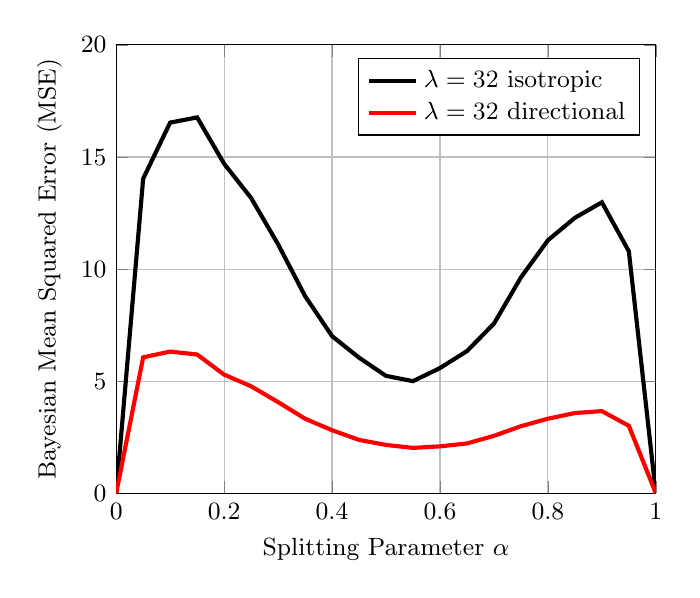
\begin{tikzpicture}
\begin{axis}[
font=\small,
xlabel= {Splitting Parameter $\alpha$},
ylabel= {Bayesian Mean Squared Error (MSE)},
xmin = 0, xmax = 1,
ymin = 0, ymax = 20,
xmajorgrids,
ymajorgrids,
legend entries={$\lambda=32$ isotropic,$\lambda=32$ directional},
legend style={legend pos=north east,nodes=right}]

% Method: Bayes,
% Area Type = inscribed,
% Antenna Type = omnidirectional,
% Noise = 2,
% Trials = 50000,
% Total rate = 16,
% alpha_step =0.025,
% A_t =36.0,
% A_o =64.0,
% BMSE

\addplot [
color=black,
line width=1.5pt,
solid,
]
coordinates{
(0,0.00000000e+00)
(0.05,1.40340910e+01)
(0.1,1.65337525e+01)
(0.15,1.67666833e+01)
(0.2,1.46989584e+01)
(0.25,1.31718747e+01)
(0.3,1.11062848e+01)
(0.35,8.79609488e+00)
(0.4,7.01012537e+00)
(0.45,6.04878165e+00)
(0.5,5.23534228e+00)
(0.55,5.00003850e+00)
(0.6,5.58474031e+00)
(0.65,6.34015503e+00)
(0.7,7.56575455e+00)
(0.75,9.62538999e+00)
(0.8,1.12850060e+01)
(0.85,1.22863272e+01)
(0.9,1.29794969e+01)
(0.95,1.07916156e+01)
(1,1.63496156e-30)
};

% Method: Bayes,
% Area Type = inscribed,
% Antenna Type = directional,
% Noise = 2,
% Trials = 50000,
% Total rate = 16,
% alpha_step =0.025,
% A_t =36.0,
% A_o =64.0,
% BMSE


\addplot [
color=red,
line width=1.5pt,
solid,
]
coordinates{
	(0,0.00000000e+00)
	(0.05,6.06211129e+00)
	(0.1,6.31985246e+00)
	(0.15,6.18877686e+00)
	(0.2,5.29187935e+00 )
	(0.25,4.77082541e+00)
	(0.3,4.06549571e+00)
	(0.35,3.32541741e+00)
	(0.4,2.81081943e+00)
	(0.45,2.37943353e+00)
	(0.5,2.15498374e+00)
	(0.55,2.02272270e+00)
	(0.6,2.09148122e+00)
	(0.65,2.22126422e+00)
	(0.7,2.56077071e+00)
	(0.75,2.98972505e+00)
	(0.8,3.32440510e+00)
	(0.85,3.57826746e+00)
	(0.9,3.66298963e+00)
	(0.95,3.00728985e+00)
	(1,1.66676843e-30)
};

\end{axis}

\end{tikzpicture}

}
	\caption{This graph shows the Bayesian mean squared error as functions of splitting parameter under the scheme of \ref{section:BayesEstimation}.
		The black line corresponds to performance of the system equipped with isotropic antennas, whereas the red line corresponds to the performance of systems with directional antennas.}
	\label{figure: BayesRt}
\end{figure}

According to Fig.~\ref{figure: BayesRt}, systems with directional antennas perform better than systems with isotropic antennas.

To further compare the performances, we introduce confidence intervals.
A confidence level refers to the percentage of all possible samples that can be expected to include the true population parameter~\cite{altman2013statistics}.
Suppose we use the same sampling method to select different samples and to compute a different interval estimate for each sample.
Some interval estimates would include the true population parameter and some may not.
A 95\% confidence level means that 95\% of the intervals would include the true parameter.
Generally, the confidence interval is computed as below.
Select a confidence level which describes the uncertainty of a sampling method.
Compute
\begin{equation*}
\gamma = 1 - (\text{confidence level} / 100) .
\end{equation*}
Find the critical probability $p^*$
\begin{equation*}
p^* = 1 - \gamma/2 .
\end{equation*}
Express the critical value as a $t$-statistic by using the degree of freedom and the critical probability, where the degree of freedom is equal to
\begin{equation*}
df = N-1
\end{equation*}
and $N$ is the sample size.
The standard error $SE$ is given as
\begin{equation*}
SE= \dfrac{\sigma}{\sqrt{N}}
\end{equation*}
where $\sigma$ is the standard deviation of the sample.
The margin of error is the product of the critical value $t^*$ and $SE$.
The confidence interval is expressed as
\begin{equation*}
\text{Confidence interval} = \mu \pm \text{Margin of error}
\end{equation*}
where $\mu$ is the mean of the sample.
In this simulation, we analyze the absolute difference between the true number of target devices $r_{t}$ and the estimated result $\hat{r_{t}}$.
The confidence intervals of $|r_{t}-\hat{r_{t}}|$ corresponding to isotropic antennas and directional antennas are summarized in Table~\ref{table:ConfidenceBayes}.
The result is based on fifty thousand samples.
\begin{table}[bht]
	\caption{Confidence interval of $|r_{t}-\hat{r_{t}}|$ for the simulated Bayes scheme.} \label{table:ConfidenceBayes}
	\centerline{
		\begin{tabular}{|l|l|c|}
			\hline
			\multicolumn{1}{|c|}{\textbf{Antenna type}} &
			\multicolumn{1}{|c|}{\textbf{Confidence interval}}&
			\multicolumn{1}{|c|}{\textbf{Confidence level}} \\
			\hline
			Directional & $1.412411 \pm 0.002166$&95\% \\
			\hline
			Isotropic & $2.454623 \pm 0.003450$&95\% \\
			\hline
		\end{tabular}}
	\end{table}
To make the result more straightforward, we use a Gaussian kernel density estimation to plot the approximation of the probability density function of $|r_{t}-\hat{r_{t}}|$.
The horizontal axis represents value for $|r_{t}-\hat{r_{t}}|$.
\begin{figure}[]
	\centering
	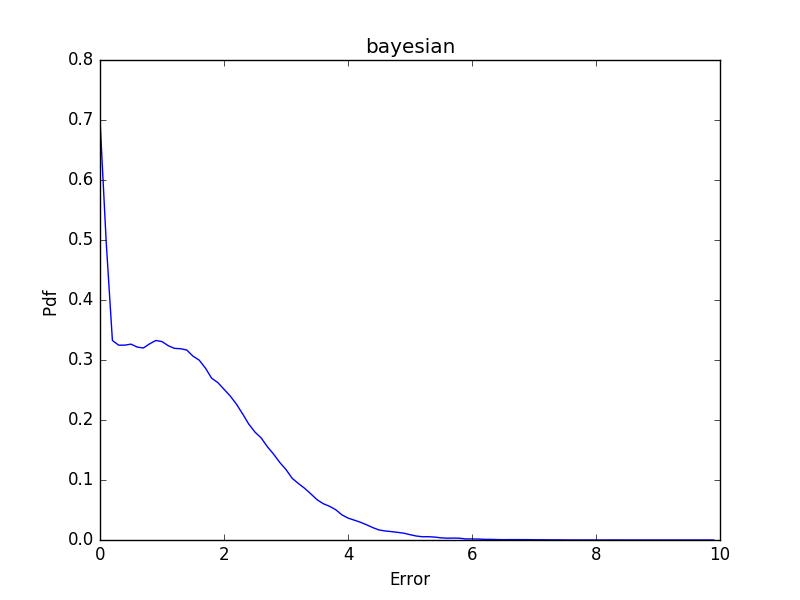
\includegraphics[scale=0.5]{Figures/bayesrtdir.png}
	\caption{This graph shows the approximation probability density function of $|r_{t}-\hat{r_{t}}|$ corresponding to the system equipped with directional antennas under the scheme of Section~\ref{section:BayesEstimation}. }
	\label{figure: BayesRtdir}
\end{figure}
\begin{figure}[]
	\centering
	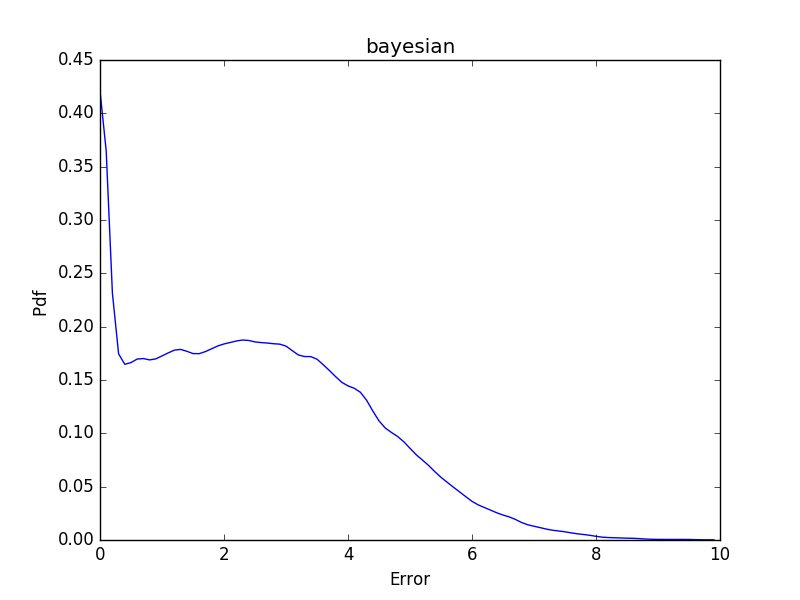
\includegraphics[scale=0.5]{Figures/bayesrtomni.png}
	\caption{This graph shows the approximation probability density function of $|r_{t}-\hat{r_{t}}|$ corresponding to the system equipped with isotropic antennas under the scheme of Section~\ref{section:BayesEstimation}. }
	\label{figure: BayesRtomni}
\end{figure}
Comparing the PDF curves in Fig.~\ref{figure: BayesRtdir} and Fig.~\ref{figure: BayesRtomni}, the distribution of the error occurs in system with directional antennas appears closer to zero.
This result, along with fact that the BMSE of directional systems is smaller, shows that systems with directional antennas perform better.
This performance improvement results from the directional antennas being more discriminating than the isotropic antennas. 


\subsection{Maximum Likelihood Estimation}

In this section, we look into the maximum likelihood estimation framework mentioned in Section~\ref{section:Maxestimation}.
We use the average mean squared error to evaluate the performance of our estimator.
As before, the total Poisson rates is set to be 32 and the curves are functions of splitting coefficient $\alpha$.
\begin{figure}[t]
	\centerline{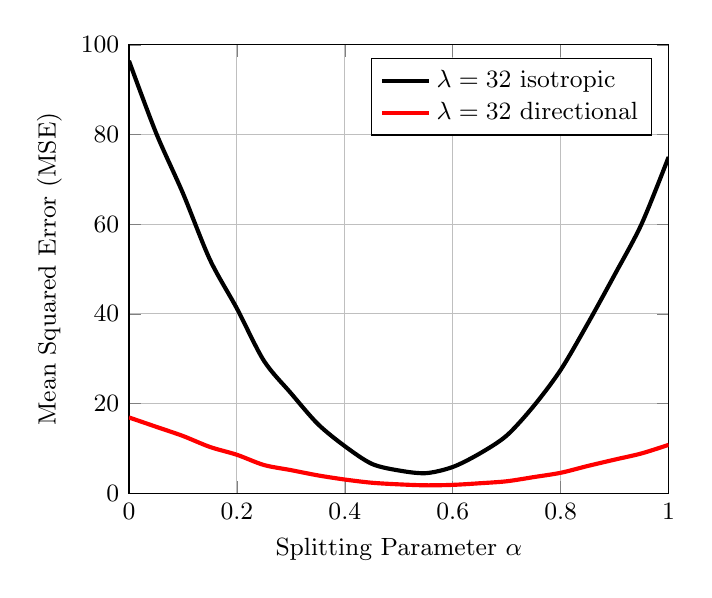
\begin{tikzpicture}
\begin{axis}[
font=\small,
xlabel= {Splitting Parameter $\alpha$},
ylabel= {Mean Squared Error (MSE)},
xmin = 0, xmax = 1,
ymin = 0, ymax = 100,
xmajorgrids,
ymajorgrids,
legend entries={$\lambda=32$ isotropic,$\lambda=32$ directional},
legend style={legend pos=north east,nodes=right}]

% Method: Maximum likelihood,
% Area Type = inscribed,
% Antenna Type = omnidirectional,
% Noise = 2,
% Trials = 50000,
% Total rate = 32,
% alpha_step =0.05,
% A_t =36.0,
% A_o =64.0,
% MSE

\addplot [
color=black,
line width=1.5pt,
solid,smooth,
]
coordinates{
(0.0, 96.45209035)
(0.05, 80.42654262)
(0.1, 66.903744)
(0.15, 52.10264146)
(0.2, 41.20324598)
(0.25, 29.55163517)
(0.3, 22.33010006)
(0.35, 15.43733205)
(0.4, 10.49123755)
(0.45, 6.55550934)
(0.5, 5.07875978)
(0.55, 4.47613893)
(0.6, 5.85587843)
(0.65, 8.86221142)
(0.7, 12.88023637)
(0.75, 19.4563296)
(0.8, 27.5197941)
(0.85, 37.81174437)
(0.9, 48.74165857)
(0.95, 60.08816203)
(1.0, 74.99918686)
};

% Method: Maximum likelihood,
% Area Type = inscribed,
% Antenna Type = directional,
% Noise = 2,
% Trials = 50000,
% Total rate = 32,
% alpha_step =0.05,
% A_t =36.0,
% A_o =64.0,
% MSE


\addplot [
color=red,
line width=1.5pt,
solid,smooth,
]
coordinates{
	(0.0, 16.90429818)
	(0.05, 14.83771601)
	(0.1, 12.77276452)
	(0.15, 10.3230366)
	(0.2, 8.5767891)
	(0.25, 6.30075548)
	(0.3, 5.15896029)
	(0.35, 3.98470553)
	(0.4, 3.05483395)
	(0.45, 2.34139352)
	(0.5, 1.98255413)
	(0.55, 1.76749939)
	(0.6, 1.86673371)
	(0.65, 2.22515382)
	(0.7, 2.66910387)
	(0.75, 3.59868373)
	(0.8, 4.56054986)
	(0.85, 6.07758196)
	(0.9, 7.49693503)
	(0.95, 8.88671712)
	(1.0, 10.7925513)
};

\end{axis}

\end{tikzpicture}

}
	\caption{This figure shows the mean squared error as functions of splitting parameter under scheme of Section~\ref{section:Maxestimation}.
		The black line corresponds to the performance of a system equipped with isotropic antennas, whereas the red line corresponds to the performance of a system with directional antennas.}
	\label{figure: MaxRt}
\end{figure}
The black curve in Fig.~\ref{figure: MaxRt} shows the MSE when the maximum likelihood estimator operates on data collected using isotropic antennas.
The red curve in Fig.~\ref{figure: MaxRt} corresponds to the scenario where the estimator operates on data collected by directional antennas.
The four directional antennas are located at the four corners of the target area, and they are pointing directly towards the center.
These antennas have a 3~dB beam-width of $\theta_{\mathrm{3dB}} = 90^{\circ}$ and a nominal attenuation floor of $G_{\mathrm{floor}} = 20$~dB.
Every point is obtained by averaging over fifty thousand trials.
The MSE is smaller for systems using directional antennas.

The confidence interval of the absolute error $|r_{t}-\hat{r_{t}}|$ corresponding to the isotropic antennas and the directional antennas are summarized in Table~\ref{table:ConfidenceMax}.
\begin{table}[bht]
	\caption{Confidence interval of $|r_{t}-\hat{r_{t}}|$ for simulation corresponding to the Maximum likelihood scheme.} \label{table:ConfidenceMax}
	\centerline{
		\begin{tabular}{|l|l|c|}
			\hline
			\multicolumn{1}{|c|}{\textbf{Antenna type}} &
			\multicolumn{1}{|c|}{\textbf{Confidence interval}} &
			\multicolumn{1}{|c|}{\textbf{Confidence level}} \\
			\hline
			Directional & $2.080484 \pm 0.002809$&95\% \\
			\hline
			Isotropic & $4.972427 \pm 0.006020$&95\% \\
			\hline
		\end{tabular}}
\end{table}
\begin{figure}[]
	\centering
	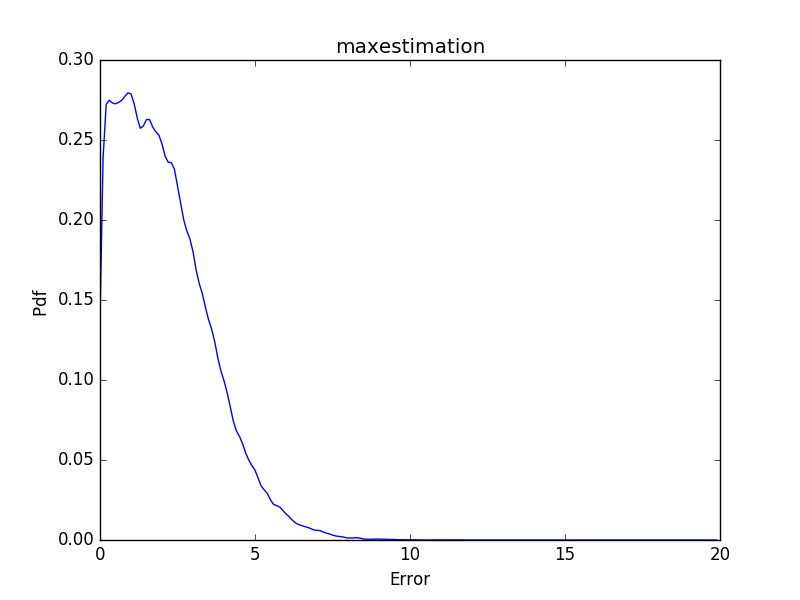
\includegraphics[scale=0.5]{Figures/maxrtdir.png}
	\caption{This graph shows the approximation probability density function of $|r_{t}-\hat{r_{t}}|$ corresponding to system equipped with directional antennas under scheme of \ref{section:Maxestimation}. }
	\label{figure: MaxRtdir}
\end{figure}
\begin{figure}[]
	\centering
	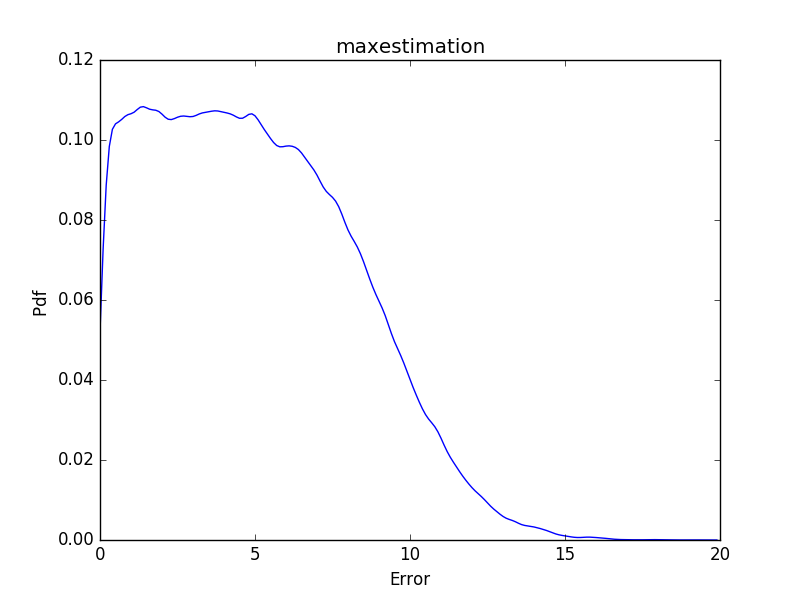
\includegraphics[scale=0.5]{Figures/maxrtomni.png}
	\caption{This graph shows the approximation probability density function of $|r_{t}-\hat{r_{t}}|$ corresponding to system equipped with isotropic antennas under scheme of \ref{section:Maxestimation}. }
	\label{figure: MaxRtomni}
\end{figure}
Comparing the PDF curves in Fig.~\ref{figure: MaxRtdir} and Fig.~\ref{figure: MaxRtomni}, we see that the distribution of the error for systems with directional antennas appears closer to zero.
This result, along with the fact that the MSE for the directional systems is smaller, shows that directional antennas outperform isotropic antennas within this context.
Again, these results indicate that the information obtained from the directional antennas is more discriminating than the that gathered by isotropic antennas. 



	\chapter{EXPERIMENTAL IMPLEMENTATION}
To complement the numerical findings based on our theoretical framework, we take an experimental implementation to assess the two schemes proposed in this work.
The RSSI signal strength data set is collected during this experiment. This information is also used to provide statistical evidence for the wireless channel model adopted
throughout. This model is used to determine the characteristics of the environment. The system is designed to work on the 2.4~GHz ISM radio band, which is used by Wi-Fi technology. In this experiment, all the wireless clients are connected to a wireless access point.
This chapter details the way the experiments are designed, and it explains the
analysis of the gathered information.


\section{Monitoring Devices}

Every sensing device takes the form of a Next Unit of Computing (NUC) by Intel{\texttrademark}, and runs the Ubuntu 14.04 operation system.
Wireless monitoring is enabled through an Alfa{\texttrademark}~\texttt{AWUS036NHA} wireless interface with a detachable antenna.
The Atheros{\texttrademark} chipset is able to listen to transmission packets on a channel if monitoring mode is turned on.
The sub-miniature version A (SMA) antenna connectors are used to attach either isotropic antennas or directional antennas.
Each monitoring device is equipped with one directional antenna and one isotropic antenna.
Wooden sticks are also employed to fix the two antennas attached to a monitoring devices, and they are positioned at different heights to reduce the interactions and the coupling effect between the two antennas.
The radiation pattern of the directional antenna is shown in Fig.~\ref{figure:Directionalantenna}.
\begin{figure}[t]
	\centerline{\begin{tikzpicture}
\begin{polaraxis}[
%scale only axis,
width=7cm,
xticklabel=$\pgfmathprintnumber{\tick}^\circ$,
y coord trafo/.code=\pgfmathparse{#1+24},
ytick={-20, -12, 0},
ymin=-25, ymax=4,
y coord inv trafo/.code=\pgfmathparse{#1-24},
%height=5cm,
%xlabel={Angle (degree)},
%ylabel={Gain (dB)},
every tick label/.append style={font=\small},
legend entries={\scriptsize{Directional},
},
legend style={at={(-0.1,0.15)}, nodes=right}
]

% Isotropic
\addplot [
color=black,
densely dotted,
line width=1.5pt
]
coordinates{
(-180,-13.4414512682882)
(-179,-13.4546700300579)
(-178,-13.4764252161895)
(-177,-13.5066749182237)
(-176,-13.5454091452149)
(-175,-13.5926512614262)
(-174,-13.6484593103953)
(-173,-13.7129271845231)
(-172,-13.786185598773)
(-171,-13.8684028282442)
(-170,-13.9597851720984)
(-169,-14.0605771102312)
(-168,-14.171061123622)
(-167,-14.2915571537574)
(-166,-14.4224216799846)
(-165,-14.564046395037)
(-164,-14.7168564570345)
(-163,-14.8813082895423)
(-162,-15.0578868880923)
(-161,-15.2471025699203)
(-160,-15.4494870710865)
(-159,-15.6655888485296)
(-158,-15.8959673799491)
(-157,-16.1411861664687)
(-156,-16.4018040249311)
(-155,-16.6783640994064)
(-154,-16.9713798135067)
(-153,-17.2813167120243)
(-152,-17.6085687852638)
(-151,-17.9534274140926)
(-150,-18.3160405027914)
(-149,-18.6963586762959)
(-148,-19.0940646335486)
(-147,-19.5084809568845)
(-146,-19.9384510871974)
(-145,-20.3821882119969)
(-144,-20.8370882639926)
(-143,-21.2995074098521)
(-142,-21.7645132926185)
(-141,-22.225635323862)
(-140,-22.6746644506975)
(-139,-23.1015859631804)
(-138,-23.4947613901067)
(-137,-23.841486082104)
(-136,-24.1290045299321)
(-135,-24.345937785169)
(-134,-24.4838807689049)
(-133,-24.538750169525)
(-132,-24.5114404842924)
(-131,-24.4075490242601)
(-130,-24.2362736547105)
(-129,-24.0088681874837)
(-128,-23.7371101123833)
(-127,-23.4321061663679)
(-126,-23.1035576892841)
(-125,-22.7594458246612)
(-124,-22.4060195668596)
(-123,-22.0479616840587)
(-122,-21.6886342872691)
(-121,-21.3303403105187)
(-120,-20.9745660215661)
(-119,-20.6221893280437)
(-118,-20.2736501988418)
(-117,-19.9290854147959)
(-116,-19.5884323141828)
(-115,-19.2515067852031)
(-114,-18.918060457562)
(-113,-18.5878214048584)
(-112,-18.2605219640107)
(-111,-17.9359166277138)
(-110,-17.6137924101798)
(-109,-17.29397362645)
(-108,-16.976322648047)
(-107,-16.6607378863736)
(-106,-16.3471499957831)
(-105,-16.035517069923)
(-104,-15.7258194204318)
(-103,-15.4180543715238)
(-102,-15.1122313742234)
(-101,-14.8083676376039)
(-100,-14.506484389242)
(-99,-14.2066038110712)
(-98,-13.9087466476471)
(-97,-13.6129304491279)
(-96,-13.3191683886201)
(-95,-13.0274685805737)
(-94,-12.7378338214717)
(-93,-12.4502616741834)
(-92,-12.1647448213794)
(-91,-11.8812716199649)
(-90,-11.5998267964784)
(-89,-11.3203922319979)
(-88,-11.0429477936784)
(-87,-10.7674721782015)
(-86,-10.4939437398711)
(-85,-10.2223412826925)
(-84,-9.95264480145817)
(-83,-9.68483616163374)
(-82,-9.41889971173306)
(-81,-9.15482282496653)
(-80,-8.89259636932495)
(-79,-8.63221510702225)
(-78,-8.37367802545644)
(-77,-8.11698860265535)
(-76,-7.86215501063776)
(-75,-7.60919026032084)
(-74,-7.35811229161282)
(-73,-7.10894401220511)
(-72,-6.86171328837428)
(-71,-6.61645289086147)
(-70,-6.37320039865155)
(-69,-6.13199806324974)
(-68,-5.89289263586871)
(-67,-5.65593515980614)
(-66,-5.42118073021528)
(-65,-5.18868822345142)
(-64,-4.95851999820981)
(-63,-4.73074157075047)
(-62,-4.50542126662129)
(-61,-4.2826298514338)
(-60,-4.06244014340366)
(-59,-3.84492661052946)
(-58,-3.63016495543777)
(-57,-3.41823169106094)
(-56,-3.20920371042792)
(-55,-3.00315785393204)
(-54,-2.80017047748882)
(-53,-2.60031702500869)
(-52,-2.40367160858357)
(-51,-2.21030659972392)
(-50,-2.02029223488485)
(-49,-1.83369623839114)
(-48,-1.65058346571357)
(-47,-1.47101556986747)
(-46,-1.29505069350371)
(-45,-1.12274318904406)
(-44,-0.954143368983411)
(-43,-0.789297288240012)
(-42,-0.628246560187275)
(-41,-0.471028207745463)
(-40,-0.3176745506513)
(-39,-0.168213129757901)
(-38,-0.0226666689462413)
(-37,0.118946925047271)
(-36,0.2566145248653)
(-35,0.390327707093715)
(-34,0.52008263971821)
(-33,0.64587993333766)
(-32,0.767724457304659)
(-31,0.885625122272774)
(-30,0.999594630939741)
(-29,1.10964919908268)
(-28,1.2158082492813)
(-27,1.31809408001364)
(-26,1.41653151308021)
(-25,1.51114752256122)
(-24,1.6019708487323)
(-23,1.68903160054985)
(-22,1.77236085046353)
(-21,1.85199022541475)
(-20,1.9279514979322)
(-19,2.00027618123524)
(-18,2.06899513220245)
(-17,2.13413816595322)
(-16,2.19573368562859)
(-15,2.25380833074432)
(-14,2.30838664722957)
(-13,2.35949078196381)
(-12,2.40714020429038)
(-11,2.45135145662405)
(-10,2.4921379358927)
(-9,2.52950970716712)
(-8,2.56347335044864)
(-7,2.59403184120972)
(-6,2.62118446492706)
(-5,2.64492676551581)
(-4,2.66525052727538)
(-3,2.6821437896941)
(-2,2.6955908942363)
(-1,2.70557256205164)
(0,2.71206600140163)
(1,2.71504504349215)
(2,2.71448030532699)
(3,2.71033937815481)
(4,2.70258704006228)
(5,2.69118549126542)
(6,2.67609461066265)
(7,2.65727223223051)
(8,2.63467443986141)
(9,2.6082558792568)
(10,2.57797008549462)
(11,2.54376982488378)
(12,2.50560744969799)
(13,2.46343526434591)
(14,2.41720590148354)
(15,2.36687270650855)
(16,2.3123901287964)
(17,2.25371411794659)
(18,2.19080252320585)
(19,2.12361549412707)
(20,2.05211588040985)
(21,1.97626962875452)
(22,1.89604617444716)
(23,1.81141882528301)
(24,1.72236513532894)
(25,1.99175117988582)
(26,1.53091233124645)
(27,1.42849272561821)
(29,1.21025729324901)
(30,1.09445528952659)
(31,0.974216741709544)
(32,0.849564514944864)
(33,0.720528173063555)
(34,0.587144096307417)
(35,0.449455557245233)
(36,0.307512752045061)
(37,0.161372784395877)
(38,0.0110995995431912)
(39,-0.143236133871139)
(40,-0.301557196188855)
(41,-0.463780045003785)
(42,-0.62981510055741)
(43,-0.799567088987819)
(44,-0.972935443560481)
(45,-1.1498147633239)
(46,-1.33009532786158)
(47,-1.51366366595923)
(48,-1.70040317508237)
(49,-1.89019478757868)
(50,-2.08291767850118)
(51,-2.27845000891792)
(52,-2.47666969755972)
(53,-2.67745521269372)
(54,-2.88068637523409)
(55,-3.08624516334933)
(56,-3.29401650823699)
(57,-3.50388907034674)
(58,-3.71575598517274)
(59,-3.9295155678316)
(60,-4.14507196600797)
(61,-4.36233575149249)
(62,-4.58122444145012)
(63,-4.80166294172245)
(64,-5.023583905855)
(65,-5.24692800510786)
(66,-5.47164410640298)
(67,-5.69768935692525)
(68,-5.92502917586247)
(69,-6.15363715547638)
(70,-6.38349487527737)
(71,-6.61459163447289)
(72,-6.84692410902017)
(73,-7.08049594049927)
(74,-7.31531726460218)
(75,-7.55140418729642)
(76,-7.7887782166628)
(77,-8.02746565804477)
(78,-8.26749697950575)
(79,-8.50890615371232)
(80,-8.7517299812968)
(81,-8.99600739956453)
(82,-9.24177877916908)
(83,-9.48908521016268)
(84,-9.73796777772268)
(85,-9.98846682695023)
(86,-10.2406212155298)
(87,-10.4944675528249)
(88,-10.7500394242691)
(89,-11.0073666007915)
(90,-11.2664742345827)
(91,-11.527382044853)
(92,-11.7901035004158)
(93,-12.0546450099917)
(94,-12.3210051360608)
(95,-12.5891738538252)
(96,-12.8591318832415)
(97,-13.1308501288662)
(98,-13.4042892690602)
(99,-13.6793995423239)
(100,-13.9561207834602)
(101,-14.2343827648686)
(102-14.5141058973709)
(103,-14.7952023390768)
(104,-15.0775775482592)
(105,-15.3611322951881)
(106,-15.6457651164751)
(107,-15.931375151856)
(108,-16.2178652458555)
(109,-16.5051451241594)
(110,-16.7931343660336)
(111,-17.0817647896647)
(112,-17.3709817474832)
(113,-17.660743694628)
(114,-17.9510192476875)
(115,-18.2417807953044)
(116,-18.5329935608064)
(117,-18.8245988554148)
(118,-19.1164901088089)
(119,-19.4084801405945)
(120,-19.7002580763119)
(121,-19.9913343773253)
(122,-20.2809727512362)
(123,-20.568108407892)
(124,-20.8512534776172)
(125,-21.1283927526256)
(126,-21.3968766416795)
(127,-21.6533236640386)
(128,-21.8935519309185)
(129,-22.1125670348475)
(130,-22.3046403175387)
(131,-22.4635124516099)
(132,-22.5827470152761)
(133,-22.6562324006537)
(134,-22.6787882718734)
(135,-22.6467850057595)
(136,-22.5586514104813)
(137,-22.4151496027575)
(138,-22.2193449738644)
(139,-21.9762785037077)
(140,-21.6924248400978)
(141,-21.3750610806376)
(142,-21.0316671990914)
(143,-20.6694416923696)
(144,-20.2949680530151)
(145,-19.9140279528015)
(146,-19.5315337437566)
(147,-19.1515450608419)
(148,-18.7773366811067)
(149,-18.4114918745034)
(150,-18.0560034400361)
(151,-17.7123714767822)
(152,-17.3816920394535)
(153,-17.0647342403978)
(154,-16.762005436053)
(155,-16.4738052695645)
(156,-16.2002698648214)
(157,-15.9414076250108)
(158,-15.6971280456792)
(159,-15.4672648118864)
(160,-15.2515942726462)
(161,-15.0498502072073)
(162,-14.8617356336503)
(163,-14.6869322676632)
(164,-14.5251081196561)
(165,-14.375923620256)
(166,-14.2390365851378)
(167,-14.1141062671784)
(168,-14.0007966942181)
(169,-13.8987794517061)
(170,-13.8077360389446)
(171,-13.7273599036436)
(172,-13.6573582404617)
(173,-13.5974536238536)
(174,-13.5473855327981)
(175,-13.50691181402)
(176,-13.4758101204807)
(177,-13.4538793527298)
(178,-13.4409411218528)
(179,-13.4368412440497)
(180,-13.4414512682882)

};

% Theta3dB = 60.0
\addplot [
color=white,
dashed,
line width=1.0pt
]
coordinates{
(-180, -12.6128) (-179, -12.6128) (-178, -12.6128) (-177, -12.6128)
(-176, -12.6128) (-175, -12.6128) (-174, -12.6128) (-173, -12.6128)
(-172, -12.6128) (-171, -12.6128) (-170, -12.6128) (-169, -12.6128)
(-168, -12.6128) (-167, -12.6128) (-166, -12.6128) (-165, -12.6128)
(-164, -12.6128) (-163, -12.6128) (-162, -12.6128) (-161, -12.6128)
(-160, -12.6128) (-159, -12.6128) (-158, -12.6128) (-157, -12.6128)
(-156, -12.6128) (-155, -12.6128) (-154, -12.6128) (-153, -12.6128)
(-152, -12.6128) (-151, -12.6128) (-150, -12.6128) (-149, -12.6128)
(-148, -12.6128) (-147, -12.6128) (-146, -12.6128) (-145, -12.6128)
(-144, -12.6128) (-143, -12.6128) (-142, -12.6128) (-141, -12.6128)
(-140, -12.6128) (-139, -12.6128) (-138, -12.6128) (-137, -12.6128)
(-136, -12.6128) (-135, -12.6128) (-134, -12.6128) (-133, -12.6128)
(-132, -12.6128) (-131, -12.6128) (-130, -12.6128) (-129, -12.6128)
(-128, -12.6128) (-127, -12.6128) (-126, -12.6128) (-125, -12.6128)
(-124, -12.6128) (-123, -12.6128) (-122, -12.6128) (-121, -12.6128)
(-120, -12.6128) (-119, -12.6128) (-118, -12.6128) (-117, -12.6128)
(-116, -12.6128) (-115, -12.6128) (-114, -12.6128) (-113, -12.6128)
(-112, -12.6128) (-111, -12.6128) (-110, -12.6128) (-109, -12.6128)
(-108, -12.6128) (-107, -12.6128) (-106, -12.6128) (-105, -12.6128)
(-104, -12.6128) (-103, -12.6128) (-102, -12.6128) (-101, -12.6128)
(-100, -12.6128) (-99, -12.6128) (-98, -12.6128) (-97, -12.6128)
(-96, -12.6128) (-95, -12.6128) (-94, -12.6128) (-93, -12.6128)
(-92, -12.6128) (-91, -12.6128) (-90, -12.6128) (-89, -12.6128)
(-88, -12.6128) (-87, -12.6128) (-86, -12.6128) (-85, -12.6128)
(-84, -12.6128) (-83, -12.6128) (-82, -12.6128) (-81, -12.6128)
(-80, -12.6128) (-79, -12.6128) (-78, -12.6128) (-77, -12.3761)
(-76, -11.8661) (-75, -11.3628) (-74, -10.8661) (-73, -10.3761)
(-72, -9.8928) (-71, -9.4161) (-70, -8.9461) (-69, -8.4828)
(-68, -8.0261) (-67, -7.5761) (-66, -7.1328) (-65, -6.6961)
(-64, -6.2661) (-63, -5.8428) (-62, -5.4261) (-61, -5.0161)
(-60, -4.6128) (-59, -4.2161) (-58, -3.8261) (-57, -3.4428)
(-56, -3.0661) (-55, -2.6961) (-54, -2.3328) (-53, -1.9761)
(-52, -1.6261) (-51, -1.2828) (-50, -0.9461) (-49, -0.6161)
(-48, -0.2928) (-47, 0.0239) (-46, 0.3339) (-45, 0.6372)
(-44, 0.9339) (-43, 1.2239) (-42, 1.5072) (-41, 1.7839)
(-40, 2.0539) (-39, 2.3172) (-38, 2.5739) (-37, 2.8239)
(-36, 3.0672) (-35, 3.3039) (-34, 3.5339) (-33, 3.7572)
(-32, 3.9739) (-31, 4.1839) (-30, 4.3872) (-29, 4.5839)
(-28, 4.7739) (-27, 4.9572) (-26, 5.1339) (-25, 5.3039)
(-24, 5.4672) (-23, 5.6239) (-22, 5.7739) (-21, 5.9172)
(-20, 6.0539) (-19, 6.1839) (-18, 6.3072) (-17, 6.4239)
(-16, 6.5339) (-15, 6.6372) (-14, 6.7339) (-13, 6.8239)
(-12, 6.9072) (-11, 6.9839) (-10, 7.0539) ( -9, 7.1172)
( -8, 7.1739) ( -7, 7.2239) ( -6, 7.2672) ( -5, 7.3039)
( -4, 7.3339) ( -3, 7.3572) ( -2, 7.3739) ( -1, 7.3839)
(  0, 7.3872) (  1, 7.3839) (  2, 7.3739) (  3, 7.3572)
(  4, 7.3339) (  5, 7.3039) (  6, 7.2672) (  7, 7.2239)
(  8, 7.1739) (  9, 7.1172) ( 10, 7.0539) ( 11, 6.9839)
( 12, 6.9072) ( 13, 6.8239) ( 14, 6.7339) ( 15, 6.6372)
( 16, 6.5339) ( 17, 6.4239) ( 18, 6.3072) ( 19, 6.1839)
( 20, 6.0539) ( 21, 5.9172) ( 22, 5.7739) ( 23, 5.6239)
( 24, 5.4672) ( 25, 5.3039) ( 26, 5.1339) ( 27, 4.9572)
( 28, 4.7739) ( 29, 4.5839) ( 30, 4.3872) ( 31, 4.1839)
( 32, 3.9739) ( 33, 3.7572) ( 34, 3.5339) ( 35, 3.3039)
( 36, 3.0672) ( 37, 2.8239) ( 38, 2.5739) ( 39, 2.3172)
( 40, 2.0539) ( 41, 1.7839) ( 42, 1.5072) ( 43, 1.2239)
( 44, 0.9339) ( 45, 0.6372) ( 46, 0.3339) ( 47, 0.0239)
( 48, -0.2928) ( 49, -0.6161) ( 50, -0.9461) ( 51, -1.2828)
( 52, -1.6261) ( 53, -1.9761) ( 54, -2.3328) ( 55, -2.6961)
( 56, -3.0661) ( 57, -3.4428) ( 58, -3.8261) ( 59, -4.2161)
( 60, -4.6128) ( 61, -5.0161) ( 62, -5.4261) ( 63, -5.8428)
( 64, -6.2661) ( 65, -6.6961) ( 66, -7.1328) ( 67, -7.5761)
( 68, -8.0261) ( 69, -8.4828) ( 70, -8.9461) ( 71, -9.4161)
( 72, -9.8928) ( 73, -10.3761) ( 74, -10.8661) ( 75, -11.3628)
( 76, -11.8661) ( 77, -12.3761) ( 78, -12.6128) ( 79, -12.6128)
( 80, -12.6128) ( 81, -12.6128) ( 82, -12.6128) ( 83, -12.6128)
( 84, -12.6128) ( 85, -12.6128) ( 86, -12.6128) ( 87, -12.6128)
( 88, -12.6128) ( 89, -12.6128) ( 90, -12.6128) ( 91, -12.6128)
( 92, -12.6128) ( 93, -12.6128) ( 94, -12.6128) ( 95, -12.6128)
( 96, -12.6128) ( 97, -12.6128) ( 98, -12.6128) ( 99, -12.6128)
(100, -12.6128) (101, -12.6128) (102, -12.6128) (103, -12.6128)
(104, -12.6128) (105, -12.6128) (106, -12.6128) (107, -12.6128)
(108, -12.6128) (109, -12.6128) (110, -12.6128) (111, -12.6128)
(112, -12.6128) (113, -12.6128) (114, -12.6128) (115, -12.6128)
(116, -12.6128) (117, -12.6128) (118, -12.6128) (119, -12.6128)
(120, -12.6128) (121, -12.6128) (122, -12.6128) (123, -12.6128)
(124, -12.6128) (125, -12.6128) (126, -12.6128) (127, -12.6128)
(128, -12.6128) (129, -12.6128) (130, -12.6128) (131, -12.6128)
(132, -12.6128) (133, -12.6128) (134, -12.6128) (135, -12.6128)
(136, -12.6128) (137, -12.6128) (138, -12.6128) (139, -12.6128)
(140, -12.6128) (141, -12.6128) (142, -12.6128) (143, -12.6128)
(144, -12.6128) (145, -12.6128) (146, -12.6128) (147, -12.6128)
(148, -12.6128) (149, -12.6128) (150, -12.6128) (151, -12.6128)
(152, -12.6128) (153, -12.6128) (154, -12.6128) (155, -12.6128)
(156, -12.6128) (157, -12.6128) (158, -12.6128) (159, -12.6128)
(160, -12.6128) (161, -12.6128) (162, -12.6128) (163, -12.6128)
(164, -12.6128) (165, -12.6128) (166, -12.6128) (167, -12.6128)
(168, -12.6128) (169, -12.6128) (170, -12.6128) (171, -12.6128)
(172, -12.6128) (173, -12.6128) (174, -12.6128) (175, -12.6128)
(176, -12.6128) (177, -12.6128) (178, -12.6128) (179, -12.6128)
(180, -12.6128)
};

% Theta3dB = 90.0
\addplot [
color=white,
solid,
line width=1.5pt
]
coordinates{
(-180, -14.2936) (-179, -14.2936) (-178, -14.2936) (-177, -14.2936)
(-176, -14.2936) (-175, -14.2936) (-174, -14.2936) (-173, -14.2936)
(-172, -14.2936) (-171, -14.2936) (-170, -14.2936) (-169, -14.2936)
(-168, -14.2936) (-167, -14.2936) (-166, -14.2936) (-165, -14.2936)
(-164, -14.2936) (-163, -14.2936) (-162, -14.2936) (-161, -14.2936)
(-160, -14.2936) (-159, -14.2936) (-158, -14.2936) (-157, -14.2936)
(-156, -14.2936) (-155, -14.2936) (-154, -14.2936) (-153, -14.2936)
(-152, -14.2936) (-151, -14.2936) (-150, -14.2936) (-149, -14.2936)
(-148, -14.2936) (-147, -14.2936) (-146, -14.2936) (-145, -14.2936)
(-144, -14.2936) (-143, -14.2936) (-142, -14.2936) (-141, -14.2936)
(-140, -14.2936) (-139, -14.2936) (-138, -14.2936) (-137, -14.2936)
(-136, -14.2936) (-135, -14.2936) (-134, -14.2936) (-133, -14.2936)
(-132, -14.2936) (-131, -14.2936) (-130, -14.2936) (-129, -14.2936)
(-128, -14.2936) (-127, -14.2936) (-126, -14.2936) (-125, -14.2936)
(-124, -14.2936) (-123, -14.2936) (-122, -14.2936) (-121, -14.2936)
(-120, -14.2936) (-119, -14.2936) (-118, -14.2936) (-117, -14.2936)
(-116, -14.2284) (-115, -13.8862) (-114, -13.5469) (-113, -13.2106)
(-112, -12.8773) (-111, -12.5469) (-110, -12.2195) (-109, -11.8951)
(-108, -11.5736) (-107, -11.2551) (-106, -10.9395) (-105, -10.6269)
(-104, -10.3173) (-103, -10.0106) (-102, -9.7069) (-101, -9.4062)
(-100, -9.1084) (-99, -8.8136) (-98, -8.5218) (-97, -8.2329)
(-96, -7.9469) (-95, -7.6640) (-94, -7.3840) (-93, -7.1069)
(-92, -6.8329) (-91, -6.5618) (-90, -6.2936) (-89, -6.0284)
(-88, -5.7662) (-87, -5.5069) (-86, -5.2506) (-85, -4.9973)
(-84, -4.7469) (-83, -4.4995) (-82, -4.2551) (-81, -4.0136)
(-80, -3.7751) (-79, -3.5395) (-78, -3.3069) (-77, -3.0773)
(-76, -2.8506) (-75, -2.6269) (-74, -2.4062) (-73, -2.1884)
(-72, -1.9736) (-71, -1.7618) (-70, -1.5529) (-69, -1.3469)
(-68, -1.1440) (-67, -0.9440) (-66, -0.7469) (-65, -0.5529)
(-64, -0.3618) (-63, -0.1736) (-62, 0.0116) (-61, 0.1938)
(-60, 0.3731) (-59, 0.5494) (-58, 0.7227) (-57, 0.8931)
(-56, 1.0605) (-55, 1.2249) (-54, 1.3864) (-53, 1.5449)
(-52, 1.7005) (-51, 1.8531) (-50, 2.0027) (-49, 2.1494)
(-48, 2.2931) (-47, 2.4338) (-46, 2.5716) (-45, 2.7064)
(-44, 2.8382) (-43, 2.9671) (-42, 3.0931) (-41, 3.2160)
(-40, 3.3360) (-39, 3.4531) (-38, 3.5671) (-37, 3.6782)
(-36, 3.7864) (-35, 3.8916) (-34, 3.9938) (-33, 4.0931)
(-32, 4.1894) (-31, 4.2827) (-30, 4.3731) (-29, 4.4605)
(-28, 4.5449) (-27, 4.6264) (-26, 4.7049) (-25, 4.7805)
(-24, 4.8531) (-23, 4.9227) (-22, 4.9894) (-21, 5.0531)
(-20, 5.1138) (-19, 5.1716) (-18, 5.2264) (-17, 5.2782)
(-16, 5.3271) (-15, 5.3731) (-14, 5.4160) (-13, 5.4560)
(-12, 5.4931) (-11, 5.5271) (-10, 5.5582) ( -9, 5.5864)
( -8, 5.6116) ( -7, 5.6338) ( -6, 5.6531) ( -5, 5.6694)
( -4, 5.6827) ( -3, 5.6931) ( -2, 5.7005) ( -1, 5.7049)
(  0, 5.7064) (  1, 5.7049) (  2, 5.7005) (  3, 5.6931)
(  4, 5.6827) (  5, 5.6694) (  6, 5.6531) (  7, 5.6338)
(  8, 5.6116) (  9, 5.5864) ( 10, 5.5582) ( 11, 5.5271)
( 12, 5.4931) ( 13, 5.4560) ( 14, 5.4160) ( 15, 5.3731)
( 16, 5.3271) ( 17, 5.2782) ( 18, 5.2264) ( 19, 5.1716)
( 20, 5.1138) ( 21, 5.0531) ( 22, 4.9894) ( 23, 4.9227)
( 24, 4.8531) ( 25, 4.7805) ( 26, 4.7049) ( 27, 4.6264)
( 28, 4.5449) ( 29, 4.4605) ( 30, 4.3731) ( 31, 4.2827)
( 32, 4.1894) ( 33, 4.0931) ( 34, 3.9938) ( 35, 3.8916)
( 36, 3.7864) ( 37, 3.6782) ( 38, 3.5671) ( 39, 3.4531)
( 40, 3.3360) ( 41, 3.2160) ( 42, 3.0931) ( 43, 2.9671)
( 44, 2.8382) ( 45, 2.7064) ( 46, 2.5716) ( 47, 2.4338)
( 48, 2.2931) ( 49, 2.1494) ( 50, 2.0027) ( 51, 1.8531)
( 52, 1.7005) ( 53, 1.5449) ( 54, 1.3864) ( 55, 1.2249)
( 56, 1.0605) ( 57, 0.8931) ( 58, 0.7227) ( 59, 0.5494)
( 60, 0.3731) ( 61, 0.1938) ( 62, 0.0116) ( 63, -0.1736)
( 64, -0.3618) ( 65, -0.5529) ( 66, -0.7469) ( 67, -0.9440)
( 68, -1.1440) ( 69, -1.3469) ( 70, -1.5529) ( 71, -1.7618)
( 72, -1.9736) ( 73, -2.1884) ( 74, -2.4062) ( 75, -2.6269)
( 76, -2.8506) ( 77, -3.0773) ( 78, -3.3069) ( 79, -3.5395)
( 80, -3.7751) ( 81, -4.0136) ( 82, -4.2551) ( 83, -4.4995)
( 84, -4.7469) ( 85, -4.9973) ( 86, -5.2506) ( 87, -5.5069)
( 88, -5.7662) ( 89, -6.0284) ( 90, -6.2936) ( 91, -6.5618)
( 92, -6.8329) ( 93, -7.1069) ( 94, -7.3840) ( 95, -7.6640)
( 96, -7.9469) ( 97, -8.2329) ( 98, -8.5218) ( 99, -8.8136)
(100, -9.1084) (101, -9.4062) (102, -9.7069) (103, -10.0106)
(104, -10.3173) (105, -10.6269) (106, -10.9395) (107, -11.2551)
(108, -11.5736) (109, -11.8951) (110, -12.2195) (111, -12.5469)
(112, -12.8773) (113, -13.2106) (114, -13.5469) (115, -13.8862)
(116, -14.2284) (117, -14.2936) (118, -14.2936) (119, -14.2936)
(120, -14.2936) (121, -14.2936) (122, -14.2936) (123, -14.2936)
(124, -14.2936) (125, -14.2936) (126, -14.2936) (127, -14.2936)
(128, -14.2936) (129, -14.2936) (130, -14.2936) (131, -14.2936)
(132, -14.2936) (133, -14.2936) (134, -14.2936) (135, -14.2936)
(136, -14.2936) (137, -14.2936) (138, -14.2936) (139, -14.2936)
(140, -14.2936) (141, -14.2936) (142, -14.2936) (143, -14.2936)
(144, -14.2936) (145, -14.2936) (146, -14.2936) (147, -14.2936)
(148, -14.2936) (149, -14.2936) (150, -14.2936) (151, -14.2936)
(152, -14.2936) (153, -14.2936) (154, -14.2936) (155, -14.2936)
(156, -14.2936) (157, -14.2936) (158, -14.2936) (159, -14.2936)
(160, -14.2936) (161, -14.2936) (162, -14.2936) (163, -14.2936)
(164, -14.2936) (165, -14.2936) (166, -14.2936) (167, -14.2936)
(168, -14.2936) (169, -14.2936) (170, -14.2936) (171, -14.2936)
(172, -14.2936) (173, -14.2936) (174, -14.2936) (175, -14.2936)
(176, -14.2936) (177, -14.2936) (178, -14.2936) (179, -14.2936)
(180, -14.2936)
};

% Theta3dB = 120.0
\addplot [
color=white,
dashdotted,
line width=1.0pt
]
coordinates{
(-180, -15.5024) (-179, -15.5024) (-178, -15.5024) (-177, -15.5024)
(-176, -15.5024) (-175, -15.5024) (-174, -15.5024) (-173, -15.5024)
(-172, -15.5024) (-171, -15.5024) (-170, -15.5024) (-169, -15.5024)
(-168, -15.5024) (-167, -15.5024) (-166, -15.5024) (-165, -15.5024)
(-164, -15.5024) (-163, -15.5024) (-162, -15.5024) (-161, -15.5024)
(-160, -15.5024) (-159, -15.5024) (-158, -15.5024) (-157, -15.5024)
(-156, -15.5024) (-155, -15.5024) (-154, -15.2657) (-153, -15.0099)
(-152, -14.7557) (-151, -14.5032) (-150, -14.2524) (-149, -14.0032)
(-148, -13.7557) (-147, -13.5099) (-146, -13.2657) (-145, -13.0232)
(-144, -12.7824) (-143, -12.5432) (-142, -12.3057) (-141, -12.0699)
(-140, -11.8357) (-139, -11.6032) (-138, -11.3724) (-137, -11.1432)
(-136, -10.9157) (-135, -10.6899) (-134, -10.4657) (-133, -10.2432)
(-132, -10.0224) (-131, -9.8032) (-130, -9.5857) (-129, -9.3699)
(-128, -9.1557) (-127, -8.9432) (-126, -8.7324) (-125, -8.5232)
(-124, -8.3157) (-123, -8.1099) (-122, -7.9057) (-121, -7.7032)
(-120, -7.5024) (-119, -7.3032) (-118, -7.1057) (-117, -6.9099)
(-116, -6.7157) (-115, -6.5232) (-114, -6.3324) (-113, -6.1432)
(-112, -5.9557) (-111, -5.7699) (-110, -5.5857) (-109, -5.4032)
(-108, -5.2224) (-107, -5.0432) (-106, -4.8657) (-105, -4.6899)
(-104, -4.5157) (-103, -4.3432) (-102, -4.1724) (-101, -4.0032)
(-100, -3.8357) (-99, -3.6699) (-98, -3.5057) (-97, -3.3432)
(-96, -3.1824) (-95, -3.0232) (-94, -2.8657) (-93, -2.7099)
(-92, -2.5557) (-91, -2.4032) (-90, -2.2524) (-89, -2.1032)
(-88, -1.9557) (-87, -1.8099) (-86, -1.6657) (-85, -1.5232)
(-84, -1.3824) (-83, -1.2432) (-82, -1.1057) (-81, -0.9699)
(-80, -0.8357) (-79, -0.7032) (-78, -0.5724) (-77, -0.4432)
(-76, -0.3157) (-75, -0.1899) (-74, -0.0657) (-73, 0.0568)
(-72, 0.1776) (-71, 0.2968) (-70, 0.4143) (-69, 0.5301)
(-68, 0.6443) (-67, 0.7568) (-66, 0.8676) (-65, 0.9768)
(-64, 1.0843) (-63, 1.1901) (-62, 1.2943) (-61, 1.3968)
(-60, 1.4976) (-59, 1.5968) (-58, 1.6943) (-57, 1.7901)
(-56, 1.8843) (-55, 1.9768) (-54, 2.0676) (-53, 2.1568)
(-52, 2.2443) (-51, 2.3301) (-50, 2.4143) (-49, 2.4968)
(-48, 2.5776) (-47, 2.6568) (-46, 2.7343) (-45, 2.8101)
(-44, 2.8843) (-43, 2.9568) (-42, 3.0276) (-41, 3.0968)
(-40, 3.1643) (-39, 3.2301) (-38, 3.2943) (-37, 3.3568)
(-36, 3.4176) (-35, 3.4768) (-34, 3.5343) (-33, 3.5901)
(-32, 3.6443) (-31, 3.6968) (-30, 3.7476) (-29, 3.7968)
(-28, 3.8443) (-27, 3.8901) (-26, 3.9343) (-25, 3.9768)
(-24, 4.0176) (-23, 4.0568) (-22, 4.0943) (-21, 4.1301)
(-20, 4.1643) (-19, 4.1968) (-18, 4.2276) (-17, 4.2568)
(-16, 4.2843) (-15, 4.3101) (-14, 4.3343) (-13, 4.3568)
(-12, 4.3776) (-11, 4.3968) (-10, 4.4143) ( -9, 4.4301)
( -8, 4.4443) ( -7, 4.4568) ( -6, 4.4676) ( -5, 4.4768)
( -4, 4.4843) ( -3, 4.4901) ( -2, 4.4943) ( -1, 4.4968)
(  0, 4.4976) (  1, 4.4968) (  2, 4.4943) (  3, 4.4901)
(  4, 4.4843) (  5, 4.4768) (  6, 4.4676) (  7, 4.4568)
(  8, 4.4443) (  9, 4.4301) ( 10, 4.4143) ( 11, 4.3968)
( 12, 4.3776) ( 13, 4.3568) ( 14, 4.3343) ( 15, 4.3101)
( 16, 4.2843) ( 17, 4.2568) ( 18, 4.2276) ( 19, 4.1968)
( 20, 4.1643) ( 21, 4.1301) ( 22, 4.0943) ( 23, 4.0568)
( 24, 4.0176) ( 25, 3.9768) ( 26, 3.9343) ( 27, 3.8901)
( 28, 3.8443) ( 29, 3.7968) ( 30, 3.7476) ( 31, 3.6968)
( 32, 3.6443) ( 33, 3.5901) ( 34, 3.5343) ( 35, 3.4768)
( 36, 3.4176) ( 37, 3.3568) ( 38, 3.2943) ( 39, 3.2301)
( 40, 3.1643) ( 41, 3.0968) ( 42, 3.0276) ( 43, 2.9568)
( 44, 2.8843) ( 45, 2.8101) ( 46, 2.7343) ( 47, 2.6568)
( 48, 2.5776) ( 49, 2.4968) ( 50, 2.4143) ( 51, 2.3301)
( 52, 2.2443) ( 53, 2.1568) ( 54, 2.0676) ( 55, 1.9768)
( 56, 1.8843) ( 57, 1.7901) ( 58, 1.6943) ( 59, 1.5968)
( 60, 1.4976) ( 61, 1.3968) ( 62, 1.2943) ( 63, 1.1901)
( 64, 1.0843) ( 65, 0.9768) ( 66, 0.8676) ( 67, 0.7568)
( 68, 0.6443) ( 69, 0.5301) ( 70, 0.4143) ( 71, 0.2968)
( 72, 0.1776) ( 73, 0.0568) ( 74, -0.0657) ( 75, -0.1899)
( 76, -0.3157) ( 77, -0.4432) ( 78, -0.5724) ( 79, -0.7032)
( 80, -0.8357) ( 81, -0.9699) ( 82, -1.1057) ( 83, -1.2432)
( 84, -1.3824) ( 85, -1.5232) ( 86, -1.6657) ( 87, -1.8099)
( 88, -1.9557) ( 89, -2.1032) ( 90, -2.2524) ( 91, -2.4032)
( 92, -2.5557) ( 93, -2.7099) ( 94, -2.8657) ( 95, -3.0232)
( 96, -3.1824) ( 97, -3.3432) ( 98, -3.5057) ( 99, -3.6699)
(100, -3.8357) (101, -4.0032) (102, -4.1724) (103, -4.3432)
(104, -4.5157) (105, -4.6899) (106, -4.8657) (107, -5.0432)
(108, -5.2224) (109, -5.4032) (110, -5.5857) (111, -5.7699)
(112, -5.9557) (113, -6.1432) (114, -6.3324) (115, -6.5232)
(116, -6.7157) (117, -6.9099) (118, -7.1057) (119, -7.3032)
(120, -7.5024) (121, -7.7032) (122, -7.9057) (123, -8.1099)
(124, -8.3157) (125, -8.5232) (126, -8.7324) (127, -8.9432)
(128, -9.1557) (129, -9.3699) (130, -9.5857) (131, -9.8032)
(132, -10.0224) (133, -10.2432) (134, -10.4657) (135, -10.6899)
(136, -10.9157) (137, -11.1432) (138, -11.3724) (139, -11.6032)
(140, -11.8357) (141, -12.0699) (142, -12.3057) (143, -12.5432)
(144, -12.7824) (145, -13.0232) (146, -13.2657) (147, -13.5099)
(148, -13.7557) (149, -14.0032) (150, -14.2524) (151, -14.5032)
(152, -14.7557) (153, -15.0099) (154, -15.2657) (155, -15.5024)
(156, -15.5024) (157, -15.5024) (158, -15.5024) (159, -15.5024)
(160, -15.5024) (161, -15.5024) (162, -15.5024) (163, -15.5024)
(164, -15.5024) (165, -15.5024) (166, -15.5024) (167, -15.5024)
(168, -15.5024) (169, -15.5024) (170, -15.5024) (171, -15.5024)
(172, -15.5024) (173, -15.5024) (174, -15.5024) (175, -15.5024)
(176, -15.5024) (177, -15.5024) (178, -15.5024) (179, -15.5024)
(180, -15.5024)
};

\end{polaraxis}
\end{tikzpicture}

}
	\caption{This graph depicts the radiation pattern of the directional antenna radiations.}
	\label{figure:Directionalantenna}
\end{figure}

A sniffing software built on the \texttt{pcap} application programming interface captures and filters wireless packets.
For filtering, we employ a hash table for removing the duplicates in the detected MAC addresses. 
The software creates a local database to store the MAC addresses and RSSI values extracted from the wireless packets observed by the system.
Finally the local database is sent to a central server for processing.
\begin{figure}[]
	\centering
	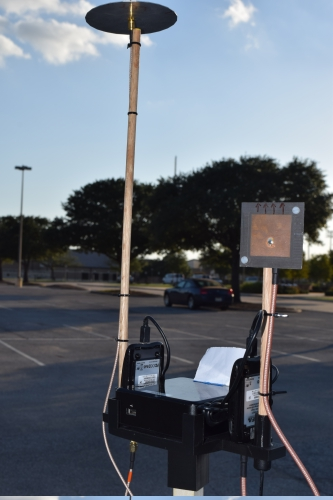
\includegraphics[scale=0.5]{Figures/DeviceSetup.jpg}
	\caption{This graph shows the monitoring device we use. }
	\label{figure: Device}
\end{figure}
The monitoring device we used during experiment is shown in Fig. \ref{figure: Device}.

\section{Wireless Client}
In our experiment, the wireless clients are Android{\texttrademark} smartphones. All the wireless clients connect to a same local access point and send packets periodically which makes them detectable by sniffing software.
For the purpose of evaluating the performance of our estimators, not only do we need RSSI values, but we also need a ground truth (i.e., the true locations of the wireless clients).
To this end, we employ a custom app, which logs GPS coordinates and time.
Throughout the experiment, the wireless clients periodically transmit their GPS information collected by the app to a central server.
MAC addresses and time stamps are subsequently employed to match locations to power vectors at the center server, yielding a data set for performance evaluation.


\section{Experimental Samples}

The experimental samples are divided into two categories, one is for monitoring devices with isotropic antennas, the other is for monitoring devices with directional antennas. Each category contains about 400 power and location vectors. Each power vector is in this form, $\underline{\mathbf{p}} = (\mathbf{p}_1, \ldots, \mathbf{p}_{4})$, where $\mathbf{p}_i$ is the power received by monitoring device~$i$.
Since there are four monitoring devices, we have almost 3200 distinct data points.

Experimental trials are then conducted as follows.
First, we generate the number of active agents inside $\r_{t}$ and number of active agents outside $\r_{o}$ according to the two Poisson distributions with parameters
\begin{xalignat*}{2}
	\lambda_{\mathrm{t}}
	&= \alpha \frac{\lambda}{A_{\mathrm{t}}}
	&\lambda_{\mathrm{o}}
	&= (1 - \alpha) \frac{\lambda}{A_{\mathrm{o}}} .
\end{xalignat*}
Then, $r_{t}$ entries are selected uniformly from clients in $A_{t}$, and $r_{o}$ entries are selected uniformly from clients in $A_{o}$.
The two collections of entries are combined into a single vector $\underline{\mathbf{p}}$, which acts as input to the estimator.
At last, the estimates are compared to the ground truth.


\section{Channel Parameters}

Channel parameters $A$ and $B$ can vary depending on the wireless environment.
This experiment is conducted on widely open parking lot.
Figure~\label{figure:Googlemap} offers a satellite image view of the experiment site.
The parameters are obtained by using the least squares method mentioned in Section~\ref{section:channel}.
The parameters for the the isotropic systems are $A = -41.68$, $B = -16.07$ and $\sigma_{s} = 7.91$~dBm.
Similarly, the parameters for the systems with directional antennas are $A = -34.72$, $B = -17.11$ and $\sigma_{s} = 8.31$~dBm.
\begin{figure}[]
	\centering
	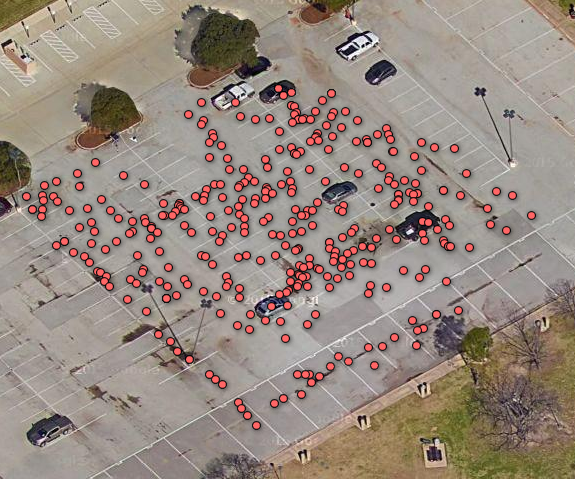
\includegraphics[scale=1]{Figures/Googlemap.png}
	\caption{This figure highlights the site used for the experiments and marks locations of experiment data. }
	\label{figure:Googlemap}
\end{figure}


\section{Experiment Results}
\subsection{Performance of Bayes Estimation}

The experimental results for the Bayes estimation scheme are shown in Fig.~\ref{figure: bayesex}.
The horizontal axis represents the splitting parameter $\alpha$.
The vertical axis corresponds to the BMSE.
Each point is averaging over 10,000 trials.
\begin{figure}[]
	\centering
	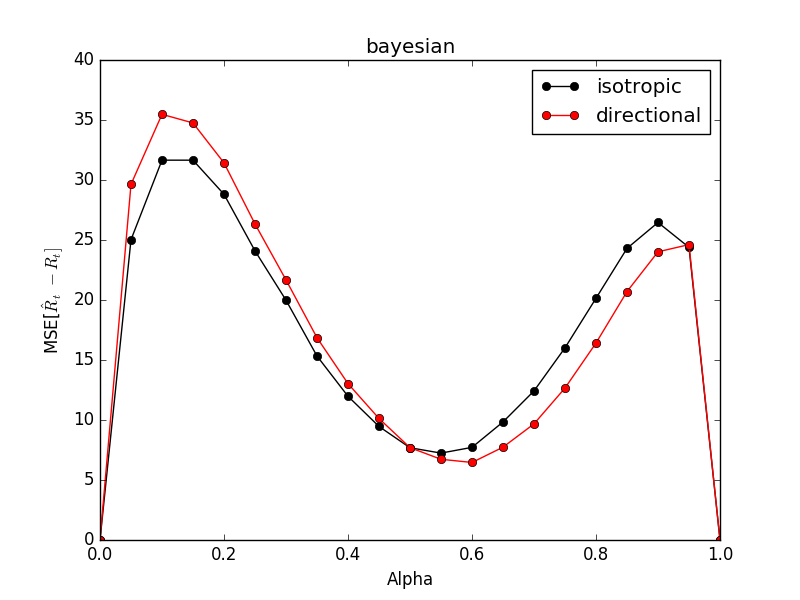
\includegraphics[scale=0.5]{Figures/bayesex.png}
	\caption{This figure depicts the experimental Bayesian mean squared error as function of Poisson splitting coefficient $\alpha$. Red line represents systems with directional antennas, whereas black line represent system with isotropic antennas. }
	\label{figure: bayesex}
\end{figure}
The confidence intervals of $|r_{t}-\hat{r_{t}}|$ corresponding to isotropic antennas and directional antennas are summarized in Table \ref{table:ConfidenceBayesex}.
\begin{table}[bht]
	\caption{Confidence interval of $|r_{t}-\hat{r_{t}}|$ for experimental Bayes scheme} \label{table:ConfidenceBayesex}
	\centerline{
		\begin{tabular}{|l|l|c|}
			\hline
			\multicolumn{1}{|c|}{\textbf{Antenna type}} &
			\multicolumn{1}{|c|}{\textbf{Confidence interval}} &
			\multicolumn{1}{|c|}{\textbf{Confidence level}} \\
			\hline
			Directional & $3.317535 \pm 0.010430$& 95\% \\
			\hline
			Isotropic & $3.331094 \pm 0.010274$ & 95\% \\
			\hline
		\end{tabular}}
	\end{table}
The approximation probability density functions corresponding to systems with directional antennas and isotropic antennas are shown in Fig. \ref{figure: bayesdirex} and Fig. \ref{figure: bayesomniex}.
\begin{figure}[]
	\centering
	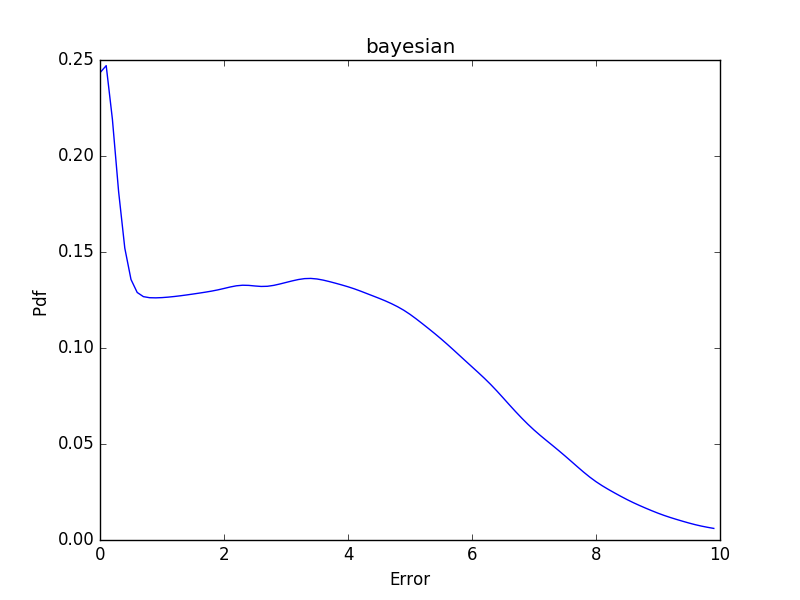
\includegraphics[scale=0.5]{Figures/bayesdirex.png}
	\caption{This graph shows the approximation probability density function of $|r_{t}-\hat{r_{t}}|$ corresponding to system equipped with directional antennas under scheme of \ref{section:BayesEstimation}. }
	\label{figure: bayesdirex}
\end{figure}
\begin{figure}[]
	\centering
	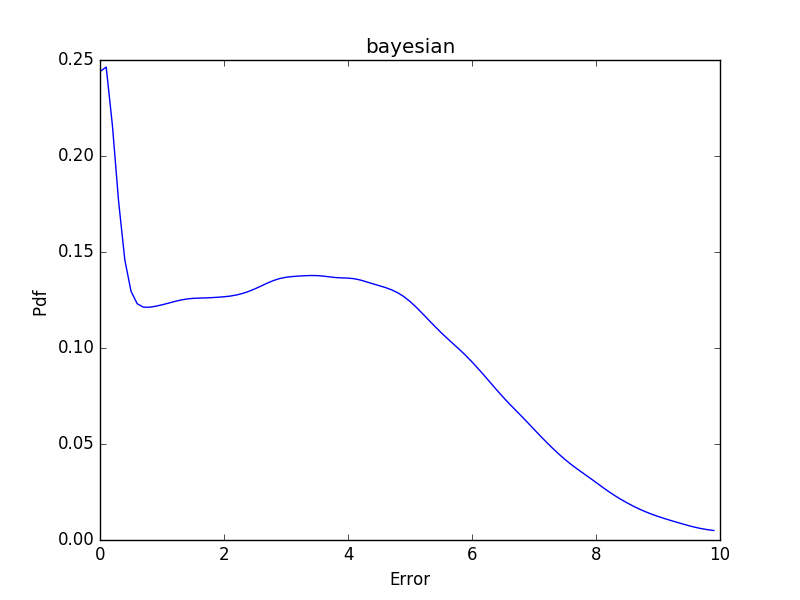
\includegraphics[scale=0.5]{Figures/bayesomniex.png}
	\caption{This graph shows the approximation probability density function of $|r_{t}-\hat{r_{t}}|$ corresponding to system equipped with isotropic antennas under scheme of \ref{section:BayesEstimation}. }
	\label{figure: bayesomniex}
\end{figure}
In this case using directional antennas does not bring an obvious benefit. The BMSE of systems with directional antennas and that with isotropic antennas are very close. As well as the confidence intervals and the absolute error distribution. This phenomena maybe caused by the inaccuracy of GPS information. Some small location errors may bring large errors, especially for the case when using directional antennas. 
\subsection{Performance of Maximum Estimation}
Experimental curves under Bayes estimation scheme is shown in Fig. \ref{figure: maxRTex}. The horizontal axis is the splitting parameter $\alpha$. The vertical axis is the BMSE. Each point is averaging over 10000 trails.
\begin{figure}[]
	\centering
	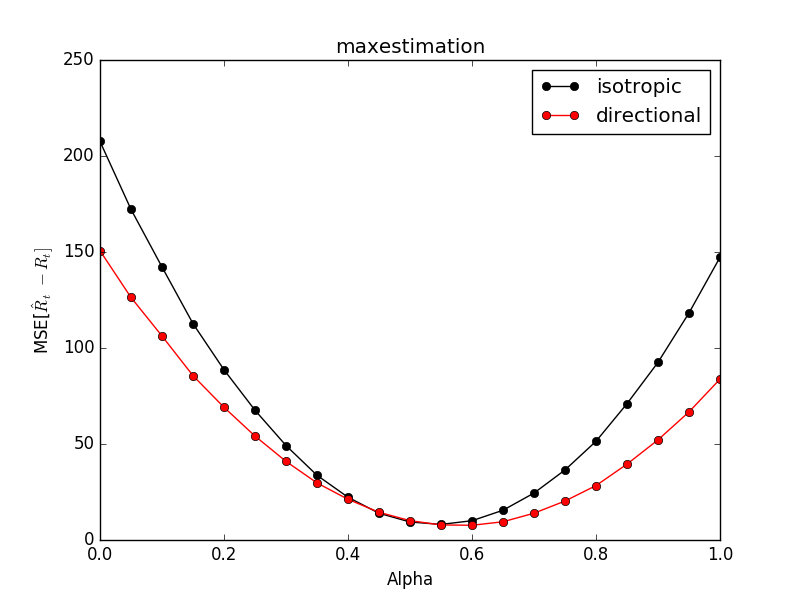
\includegraphics[scale=0.5]{Figures/maxRTex.png}
	\caption{This figure depicts the experimental Bayesian mean squared error as function of Poisson splitting coefficient $\alpha$. Red line represents systems with directional antennas, whereas black line represent system with isotropic antennas. }
	\label{figure: maxRTex}
\end{figure}
The confidence intervals of $|r_{t}-\hat{r_{t}}|$ corresponding to isotropic antennas and directional antennas are summarized in Table \ref{table:Confidencemaxex}.
\begin{table}[bht]
	\caption{Confidence interval of $|r_{t}-\hat{r_{t}}|$ for experimental Maximum estimation scheme} \label{table:Confidencemaxex}
	\centerline{
		\begin{tabular}{|l|l|c|}
			\hline
			\multicolumn{1}{|c|}{\textbf{Antenna type}} &
			\multicolumn{1}{|c|}{\textbf{Confidence interval}}&
			\multicolumn{1}{|c|}{\textbf{Confidence level}} \\
			\hline
			Directional & $5.881027 \pm 0.016484$ &95\% \\
			\hline
			Isotropic & $7.144900 \pm 0.019182$ &95\% \\
			\hline
		\end{tabular}}
	\end{table}
	The approximation probability density functions corresponding to systems with directional antennas and isotropic antennas are shown in Fig. \ref{figure: maxdirex} and Fig. \ref{figure: maxomniex}.
	\begin{figure}[]
		\centering
		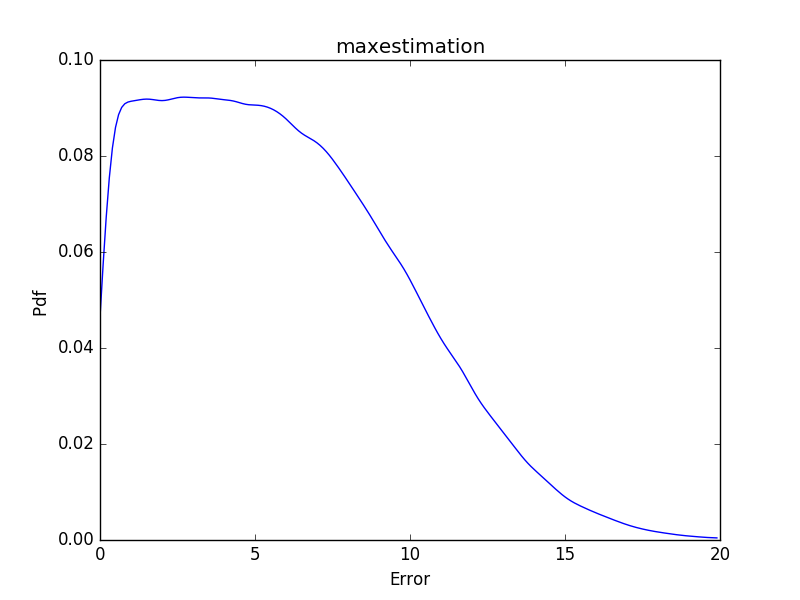
\includegraphics[scale=0.5]{Figures/maxdirex.png}
		\caption{This graph shows the approximation probability density function of $|r_{t}-\hat{r_{t}}|$ corresponding to system equipped with directional antennas under scheme of \ref{section:Maxestimation}. }
		\label{figure: maxdirex}
	\end{figure}
	\begin{figure}[]
		\centering
		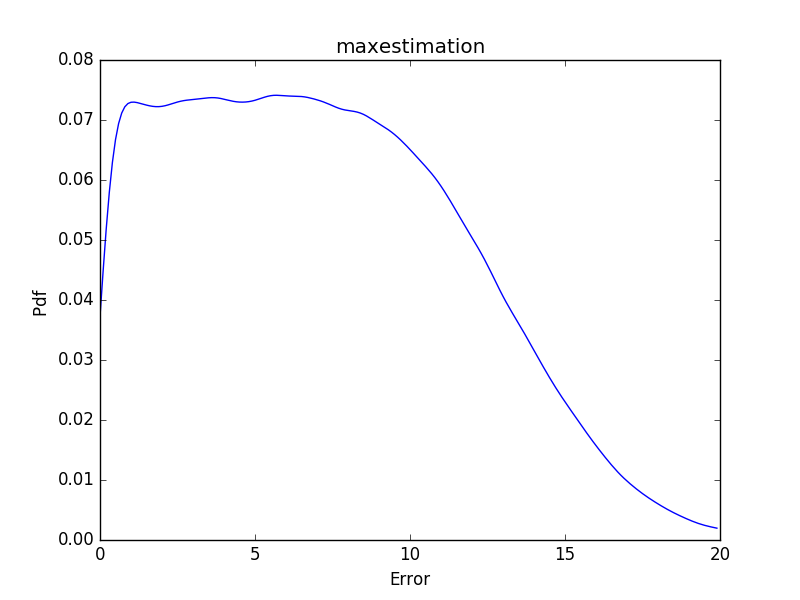
\includegraphics[scale=0.5]{Figures/maxomniex.png}
		\caption{This graph shows the approximation probability density function of $|r_{t}-\hat{r_{t}}|$ corresponding to system equipped with isotropic antennas under scheme of \ref{section:Maxestimation}. }
		\label{figure: maxomniex}
	\end{figure}
In this case, systems with directional antennas better, which means systems equipped with direcional antennas are more discrimination.

	\chapter{CONCLUSION}
\ignore{This work will include a numerical simulation corresponding to two estimation schemes. The simulation code is written in python. The simulation will show the performance comparison between directional antenna and isotropic antenna. The performance is evaluated via estimation error(BMSE for Bayesian estimation and MSE for maximum likelihood estimation). Preliminary results shows that performance improved when using directional antennas. To further support this result, an experiment will be conducted in the line of sight areas to obtain the experimental data. The performance of estimation will be reported with the experimental data obtained.}
		
\TAMUReferenceFormat
	\bibliographystyle{ieeetr}
	\bibliography{data/myReference}

	
\appendix
\TAMUAppendixFormat		
%comment the line below if using ChapterMethod or there is no Appendix
\begin{appendices}

%keep this line always if you have appendix
	\chapter{MISCELLANEOUS \label{cha:appendix}}

\section{Figures/Tables in Appendix}

%\begin{figure}[ht]
%\centering
%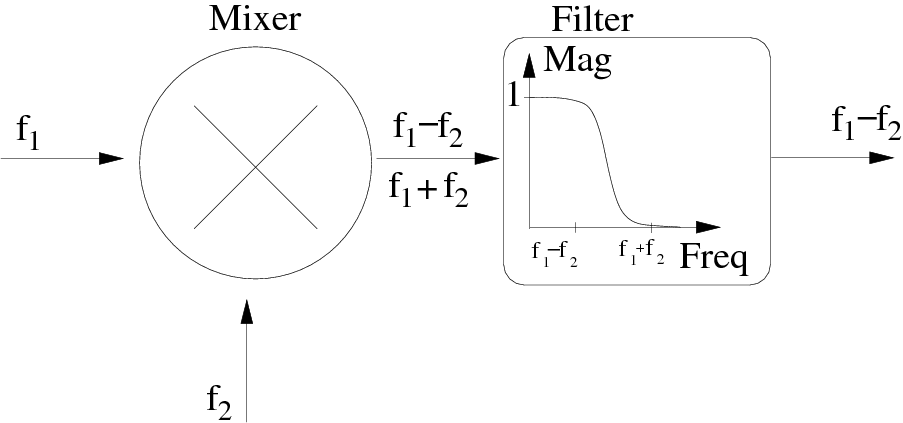
\includegraphics[scale=0.50]{analogue_mixer.png}
%\caption{Test Picture for lof (List of Figures) Display Test Purpose Only
%[The file used is in PDF format.]}

%\label{fig:A.1}

%\end{figure}

%\begin{figure}[ht]
%\centering
%\includegraphics[scale=0.60]{TestPattern1.bmp}
%\caption{CS4270 Test Bench 1 FPGA Design Diagram
%[Picture is for test display purpose only. No meaning.]}

%\label{fig:A.2}

%\end{figure}

% Add this code if you want to get the "Page" word on top of the TOC for the corresponding page. 
%\addtocontents{toc}{\protect\afterpage{~\hfill{Page}\par\medskip}}

\subsection{TEST1}
Test subsection for toc display purpose only.

%\begin{figure}[ht]
%\centering
%\includegraphics[scale=0.90]{TESTOUT3_2bit_2.bmp}
%\caption{Behavioral simulation for TEST1
%[Picture is for test display purpose only. No meaning.]}

%\label{fig:A.3}

%\end{figure}

\subsection{TEST2}
\begin{lstlisting}[language={Verilog},tabsize=12,]
  Begin
     
      If ( shift == 1'b1)
         Begin
         
         sr[(N-1):1] <= sr[(N-2):0];
sr[0] <= sr_in;
end
else
begin
sr[(N-1):1] <= sr[(N-2):0];
sr[0] <= sr[(N-1)];
end
end
\end{lstlisting}

\section{Random Pictures and Test}
Section here is to test toc display purpose only.

\section{Misc Test}
Section here is to test toc display purpose only.

\chapter{SOURCE CODE}

**Some text here**

\section{Misc Test 2}
Section here is to test toc display purpose only.

\section{Misc Test 3}
Section here is to test toc display purpose only.

\section{Resource Usage}
\begin{landscape}
\noindent
Design Summary (This page shows how to use landscape format in Appendix.)\\
\texttt{---------}\\
Design Summary:\\
Number of errors: 0\\
Number of warnings: 0\\
Logic Utilization:\\
Number of Slice Flip Flops: 3,899 out of 33,280 11\%\\
Number of 4 input LUTs: 3,717 out of 33,280 11\%\\
Logic Distribution:\\
Number of occupied Slices: 2,198 out of 16,640 13\%\\
Number of Slices containing only related logic: 2,198 out of 2,198 100\%\\
Number of Slices containing unrelated logic: 0 out of 2,198 0\%\\
*See NOTES below for an explanation of the effects of unrelated logic.\\
Total Number of 4 input LUTs: 3,890 out of 33,280 11\%\\

\end{landscape}


\begin{landscape}
\begin{table}[htbp]


 \label{table:B.1}
 
 \caption{Summary of Equipment Used}
 
\begin{tabular}{|c|c|c|}
\hline
\textbf{NAME} & \textbf{NO}. & \textbf{COMMENT}\\
\hline
Tektronix TDS7704B Scope & 1 & 7GHz, 20GSa/s time-equivallent sampling oscilloscope\\
\hline
Tektronix P7240 Probe & 2 & 4GHz Single Ended Active Probe(High Impedance)\\
\hline
Agilent 81130A Function Generator & 1 & 2 CHs Signal Generator \\
\hline
Xilinx Spartan-3A DSP 1800A Demo Board & 1 & \url{http://goo.gl/Svvpy}\\
\hline

\end{tabular}
\begin{tablenotes} 
\small 
\item
\relax
[By University Requirement, no text should be allowed here in this landscape table/picture page. \textbf{DON'T USE sidewaystable from rotating package, it cannot align landscape title to the left binding side.]} 
\end{tablenotes}
\end{table}
\end{landscape}


	
%comment the line below if using ChapterMethod or no Appendix
\end{appendices}


\end{document}
